\documentclass{article}

\usepackage[utf8]{inputenc}
\usepackage[T1]{fontenc}
\usepackage{amsmath}
\usepackage{amsfonts}
\usepackage{amssymb}
\usepackage{graphicx, booktabs}
\usepackage{authblk}
\usepackage{fullpage}
\usepackage{subfigure}
\usepackage{color}
\usepackage{hyperref}
\usepackage{mathtools}
\usepackage{threeparttable}
\usepackage[figuresright]{rotating}

\usepackage{mathptmx}
\usepackage{mathrsfs}
%\usepackage{url}

\usepackage[super,numbers]{natbib}
\bibliographystyle{abbrvnat}
\usepackage{xltabular}
\usepackage{tcolorbox}

\usepackage{siunitx}
\sisetup{range-phrase=--, range-units=single}

\graphicspath{{img/}}



\title{Advancing Treatment of Retinal Disease through \textit{in silico} Trials}

% \author[1,2]{R\'emi Hernandez}
% \author[3]{Paul A. Roberts}
% \author[1,2]{Wahbi K. El-Bouri}
% \affil[1]{Liverpool Centre for Cardiovascular Science, University of Liverpool and Liverpool Heart \& Chest Hospital Liverpool, UK}
% \affil[2]{Department of Cardiovascular and Metabolic Medicine, University of Liverpool, UK}
% \affil[3]{Centre for Systems Modelling and Quantitative Biomedicine, University of Birmingham, UK}
% \date{}


\author[1,2]{R\'{e}mi Hernandez\footnote{E-mail address: remi.hernandez@liverpool.ac.uk (R\'{e}mi Hernandez)}}
\author[3]{Paul A. Roberts\footnote{E-mail address: p.a.roberts@univ.oxon.org (Paul A. Roberts)}}
\author[1,2]{Wahbi K. El-Bouri\footnote{E-mail address: w.el-bouri@liverpool.ac.uk (Wahbi K. El-Bouri)}}                                                                                                           
\affil[1]{Liverpool Centre for Cardiovascular Science, University of Liverpool and Liverpool Heart \& Chest Hospital Liverpool, UK}                                                                                
\affil[2]{Department of Cardiovascular and Metabolic Medicine, University of Liverpool, UK}                                                                                                                        
\affil[3]{Centre for Systems Modelling and Quantitative Biomedicine, University of Birmingham, Institute of Biomedical Research, Birmingham, B15 2TT, UK}                                                          
%                                                                                                                                                                                                                  
\renewcommand\Authands{ and }                                                                                                                                                                                      
%                                                                                                                                                                                                                  
%                                       
\begin{document}

\date{\vspace{-5ex}}
\maketitle


\begin{abstract}
Approx 250 - 300 words is fine here summarising the review
\end{abstract}

\newpage
\tableofcontents
\newpage

\section*{Glossary}\label{sec:Glossary}

\begin{xltabular}{\paperheight}{ll}
  \caption{List of abbreviations.}\\
  \toprule  % \hline
  \textbf{Term} & \textbf{Definition}                                       \\
  \midrule %\hline
  \multicolumn{2}{l}{\textit{\textbf{Mathematical terms}}}                  \\
  1/2/3D        & 1/2/3 spatial   dimensions                                \\
  ISCT          & \textit{In silico} clinical trial                       \\
  ODE           & Ordinary differential   equation                          \\
  PD/PK         & Pharmacodynamics/Pharmacokinetics                         \\
  PDE           & Partial differential equation      \\
  VP            & Virtual population                                        \\
  VVUQ          & Validation,   verification and uncertainty quantification \\
  \multicolumn{2}{l}{\textit{\textbf{Biological terms}}}                    \\
  AMD           & Age-related macular   degeneration                        \\
  BrM           & Bruch’s membrane                                          \\
  CC            & Choriocapillaris                                          \\
  CRA/CRV       & Central retinal   artery/central retinal vein             \\
  DCP           & Deep capillary plexus                                     \\
  DR            & Diabetic retinopathy                                      \\
  DRC           & Deep retinal   capillaries                                \\
  DVC           & Deep vascular complex                                     \\
  GA            & Geographic atrophy \\
  GCL & Ganglion cell layer\\
  ICP           & Intermediate   capillary plexus                           \\
  ILM           & Inner limiting   membrane                                 \\
  IOP           & Intraocular pressure \\
  IS            & Inner segment(s)                                          \\
  IVI           & Intravitreal   injection                                  \\
  LACT          & Lactate                                                   \\
  nAMD          & Neovascular AMD                                       \\
  OCT           & Optical coherence   tomography                            \\
  OCTA           & Optical coherence tomography angiography                 \\
  ONL           & Outer nuclear layer                                       \\
  OS            & Outer segment(s)                                          \\
  PO$_2$        & Partial pressure of   oxygen                              \\
  ROS           & Reactive oxygen   species                                 \\
  RP            & Retinitis   pigmentosa                                    \\
  RPE           & Retinal pigment   epithelium                              \\
  RPCP          & Radial peripapillary   capillary plexus                   \\
  SVC           & Superficial vascular   complex                            \\
  SVP           & Superficial vascular   plexus                             \\
  VEGF          & Vascular endothelial   growth factor        \\
  \bottomrule %\hline
\end{xltabular}

\section{Introduction}\label{sec:Introduction}
  
The highly detailed images our eyes are capable of capturing necessitate the close interplay and coupling of many different cells and structures.
The retina, at the back of the eye, is a complex and fragile tissue playing a major role in visual functions.
Small changes in the retina can lead to degradation of visual functions which in turn can severely affect the quality of life of patients.
As such, it is perhaps not surprising that many severe visual impairments find their root in the retina.

A number of devices exist to observe the retina and clinically relevant biomarkers, often noninvasively.
For instance, optical coherence tomography (OCT) and its angiographic extension (OCTA) enable noninvasive three dimensional, high resolution scans of the retinal structure and vessels in a matter of seconds.
These devices undoubtedly improve clinical care by providing accurate measurements of biomarkers, such as oedema, which in turn informs treatment strategies.
As these devices are noninvasive and high resolution, progression of retinal disease can be monitored with repeat scans.
Following diagnosis, treatment strategies tend to be standardized, based on successful clinical trials guidelines.
However, treatment response varies between patients, indicating that alternative or tailored treatments may be needed.
The development of new treatments or dosing strategies is long, arduous and expensive, with only a small fraction of clinical trials succeeding, mostly due to an inability to prove effectiveness~\cite{Fogel_2018}.

\textit{In silico} modelling can offer insights on the underlying causes of disease, which are often hard or impossible to obtain by experimental or observational means.
The past two decades have seen a rise in the use of such models for basic research in biology and medicine.
Furthermore, the use of digital evidence to inform clinical trials is also gaining traction. 
The recent increase in the number of literature reviews on mathematical models of the eye and the retina and the development of platforms for simulating the eye accessible to non-modellers are evidence of that interest in ophthalmology~\cite{Arciero_2019,Arciero_2017,Bhandari_2021,Harris_2013,Prudhomme_2021,Roberts_2016,Sala_2018}.

\textit{In silico} clinical trials can enhance both clinical care and traditional clinical trials, preserving sight for the fast-growing number of patients suffering from retinal disorders.
Running \textit{in silico} clinical trials requires a close collaboration between experimentalist, modellers and clinicians (see Figures~\ref{fig:ModellingCycle} and~\ref{fig:ISCT}).
Other medical disciplines such as oncology and cardiology have already benefited from \textit{in silico} trials~\cite{Gaffney2022,Ravvaz2017}.
Ophthalmology can also benefit from computer aided clinical development.
Indeed, the retina provides researchers with a wealth of images and measurements that is perhaps unparalleled in other medical specialities.

In this paper, we will review state-of-the-art models of the retina, both in health and disease, and highlight the challenges to developing \textit{in silico} clinical trials for retinal diseases.
The remainder of this paper is organized as follows.
In Section~\ref{sec:RetinalPhysiology}, we provide a brief introduction to the physiology of the retina and summarize available treatments in retinal diseases.
In Section~\ref{sec:MathematicalPrimer}, we define terms and concepts related to \textit{in silico} modelling.
Sections~\ref{sec:RetinalHaemodynamicsNAMDDR} and~\ref{Sec_Ox_RP_non-nAMD} review models of the retinal physiology in health and disease and models of the treatment of major retinal diseases.
Section~\ref{sec:DrugDelivery} is dedicated to models of therapeutic procedures.
Section~\ref{sec:InSilicoTrials} defines \textit{in silico} trials and provides the reader with examples of their successful application.
Finally, in Section~\ref{sec:Conclusion}, we summarize the state of mathematical models of the retina and provide a plan of action to achieve \textit{in silico} clinical trials for retinal pathologies.

\section{Retinal physiology and therapeutic approaches}\label{sec:RetinalPhysiology}

\subsection{Physiology}


\subsubsection{Retinal layers, cells and the visual cycle.}

The retina is a layer of tissue less than \SI{0.5}{\mm} thick that lines the back of the eye~\cite{Gupta_2015}.
The retinal inner surface is attached to the vitreous body, the clear gel that separates the lens and the retina; while its outer surface is attached to Bruch's membrane (BrM) (Figure~\ref{fig:architecture-eye}).
When looking at a cross section of the retina, as shown in Figure~\ref{fig:architecture-eye}, several layers can be identified. The innermost (closest to the vitreous) being the nerve fiber layer and the outermost being the retinal pigmented epithelium (RPE).
The layers located above the RPE are made of neurons and synapses and are collectively referred to as the neurosensory retina.
In the centre of the retina is an oval-shaped pigmented area called the macula that can be seen on photographs of the retina (Figure~\ref{fig:architecture-eye}).
The macula is about \SI{5}{\mm} wide and is responsible for highly detailed, central, vision, owing to its high concentration of photoreceptor cells, namely rods and cones.
In particular, cones are highly concentrated in the centre of the macula, in a pit approximately \SI{1.5}{\mm} wide named the fovea.
The macula is a critical area of the retina, as this is where visual acuity is highest.
The macula is also an area where a number of pathological conditions present.


\begin{figure}[t!]
  \centering
  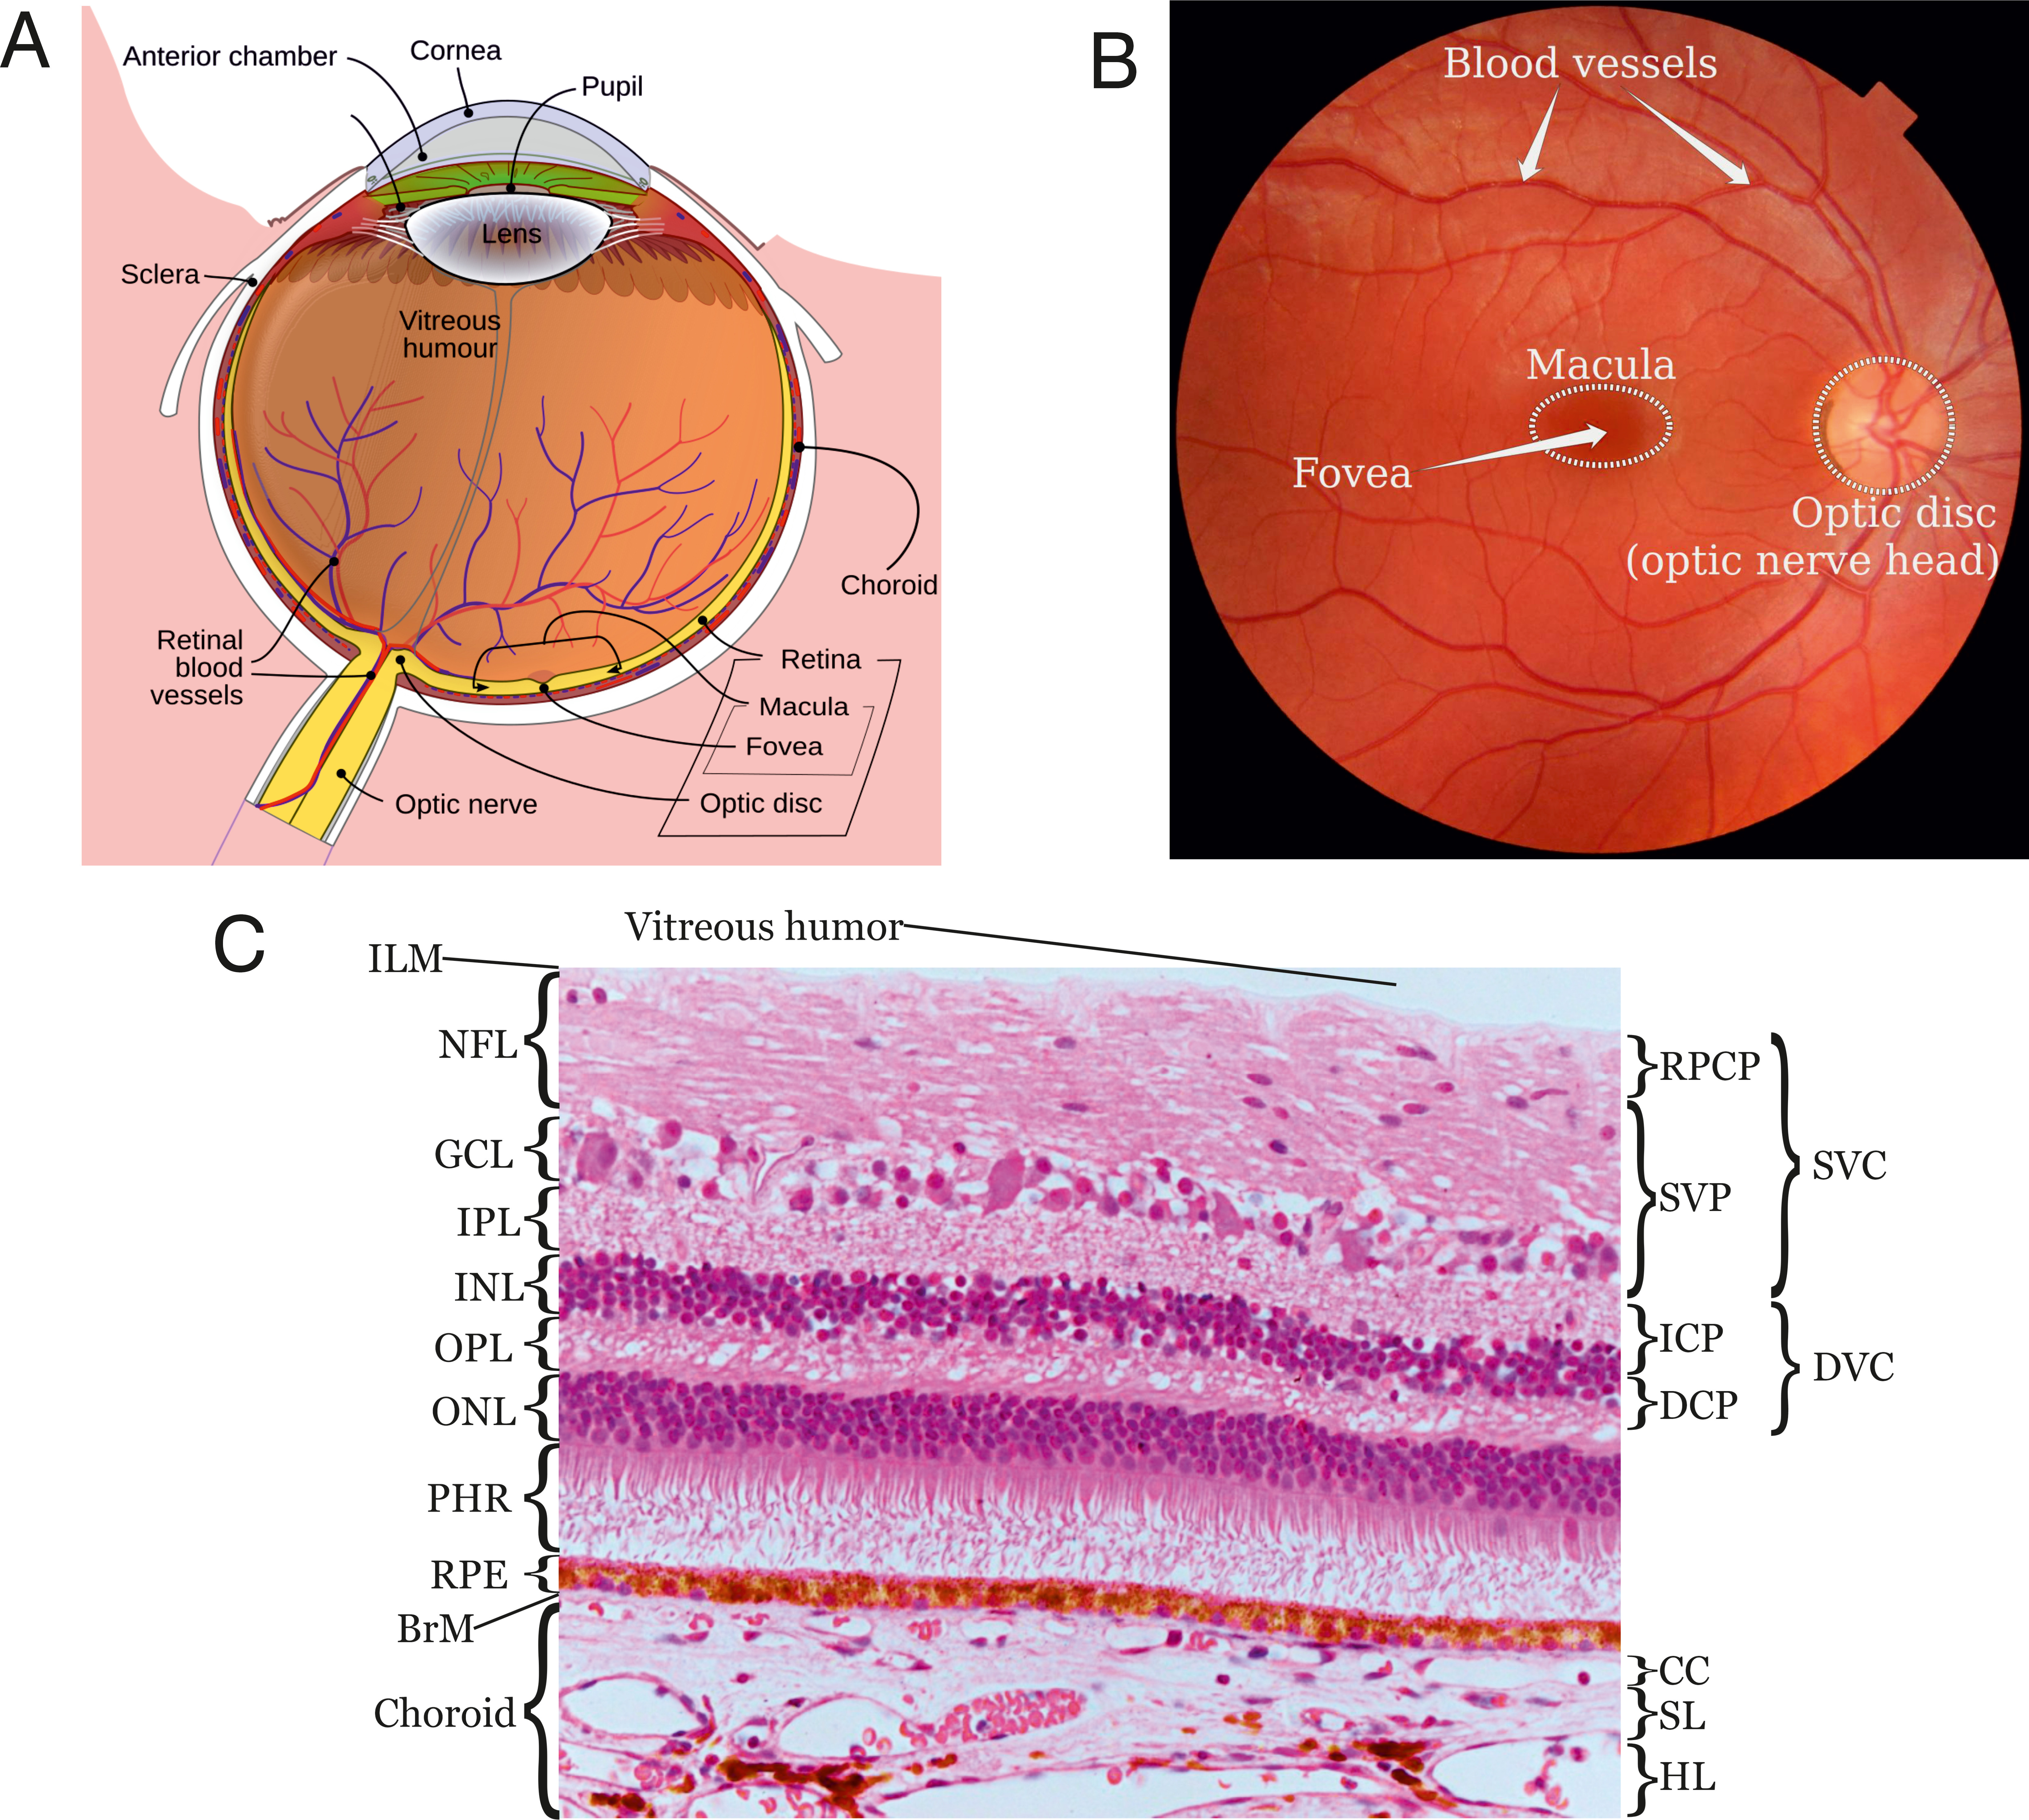
\includegraphics[width=\textwidth]{Figure1}
  \caption{Anatomy of the eye and the retina. The anatomy of the eye (A). Image credits to: Rhcastilhos and Jmarchn, distributed under CC BY-SA 3.0 license via Wikimedia Commons. Anatomical features of an healthy retina seen on a fundus photograph (B), by Mikael H\"aggstr\"om, used with permission. The retinal and choroidal layers and membranes (C). From inner retina to outer choroid: inner limiting membrane (ILM), nerve fiber layer (NFL), ganglion cell layer (GCL), inner plexiform layer (IPL), inner nuclear layer (INL), outer plexiform layer (OPL), outer nuclear layer (ONL), photoreceptors (PHR), retinal pigmented epithelium (RPE), Bruch's membrane (BrM), choriocapillaris (CC), Sattler's layer (SL), Haler's layer (HL). Modified from the work of Trivi\~no et al., published under CC BY 3.0 license.~\cite{Trivino_2012}}
  \label{fig:architecture-eye}
\end{figure}


Visual information originates from light hitting the retina.
The light crosses the inner retina to reach the photoreceptors, in the layer lying inwards from the RPE (see Figure~\ref{fig:architecture-eye}).
Activation of photoreceptors by photons starts a cascade of biochemical reactions that transforms light into a biochemical signal~\cite{Hurley_2009}.
This biochemical signal is picked up by cells in the inner layers of the retina, which transform it into an electrical signal~\cite{Arslan_2018}.
The electrical signal is then transmitted to the nerve fiber layer, which relays it to the brain via the optic nerve, enabling vision.
The optic nerve is composed of the axons of the retinal ganglion cells, amounting to between $500,000$ and $1.2$ million, and is surround by connective tissue~\cite{Salazar_2019}.
The optic nerve enters the retina through the optic disc, seen as a round spot, around \SI{1.8}{\mm} wide, on fundus photographs of the retina (Figure~\ref{fig:architecture-eye}).
The optic disc is an important structure of the retina in disease and is closely monitored by clinicians for symptoms of, e.g., glaucoma.

Owing to its pigmentation, the RPE acts as a buffer for any remaining light, protecting the retina from light damage and preventing backreflection of light that may interfere with the visual outcome.
The RPE is formed of a single layer of epithelial cells, whose primary function is to support the photoreceptors and the choroid.
To fulfill this purpose, the RPE acts as the blood-retinal barrier, regulating the transport of ions, fluid, proteins and other molecules~\cite{Boulton_2001}.

The photoreceptors abut to the RPE.
Through this close interaction, the RPE exchanges metabolites with the photoreceptors.
The RPE also transports nutrients such as retinoids to the photoreceptor cells where they are essential for the production of the light-sensitive rhodospin protein~\cite{Boulton_2001}.
By-products of the photoreceptors activity are released into the systemic circulation via the choroid, one of the two circulations of the retina~\cite{Boulton_2001}.
The cells of the RPE also play a major role in the immune response in the retina and in maintaining the choroidal vasculature through secretion of various vascular growth factors~\cite{Boulton_2001,Detrick_2020}.

\subsubsection{Blood supply to the retina}

Visual function requires high metabolic activity from the retinal cells, making the retinal tissue very oxygen demanding.
In fact, the rates of oxygen consumption per unit volume of tissue are comparable for the brain and the retina~\cite{Medrano_1995}.
To sustain the demand in oxygen, the retina is equipped with a dense network of capillaries, that branch out of the central retinal artery (CRA) and terminate at the central retinal vein (CRV).
The CRA is a branch of the ophthalmic artery and the CRV drains into the superior ophthalmic vein.
Both the CRA and CRV enter and exit the retina along the optic nerve (see Figure~\ref{fig:architecture-eye}).
The CRA's branches spread across four plexi within the inner retina, namely, the superficial vascular plexus (SVP) and the intermediate (ICP), deep (DCP) and radial peripapillary capillary plexus (RPCP).
The terms superficial vascular complex and deep vascular complex are sometimes used to designate the RPCP-SVP complex and the ICP-DCP complex, respectively.
% The inner retinal circulation provides oxygen for the inner \SIrange{60}{80}{\percent} of the tissue.
% The perfusion of the remaining outer \SIrange{20}{40}{\percent} is covered by the choroid\cite{Birol_2007}.

The choroid is a vascular tissue of the eye that lies outward from the RPE, from which it is separated by BrM.
BrM is a thin (\SIrange{2}{4}{\micro\meter}), permeable barrier that provides structural support to the RPE and regulates gas and mass exchanges with the choroid~\cite{Curcio_2013}.
The choroid is structured in three vascular layers.
From the outermost to the innermost: Haller's layer, Sattler's layer and the choriocapillaris (CC).
The diameter of the vessels in each layer decreases as it approaches the retina, with the CC composed only of capillaries, as seen on Figure~\ref{fig:architecture-eye}.
The vascular input to the choroid is provided by the short posterior ciliary arteries (between 6 and 12), which are branches of the ophthalmic artery~\cite{Kiel_2011}.
The large vessels of the two outer layers of the choroid run parallel to the retinal axis.
Some arterioles from Sattler's layer branch at an almost \SI{90}{\degree} angle to perfuse the CC~\cite{Nickla_2010}.
Each of these arterioles form an hexagonal-shaped domain, fed by a single arteriole and drained by a varying number of venules back into Sattler's layer~\cite{Zouache_2016}.
The capillaries of the CC have wide lumen (the cavity delimited by the vessel's walls), between \SIrange{7}{40}{\micro\meter} in the CC versus \SIrange{5}{10}{\micro\meter} for the retinal capillaries, and are arranged into a single plane, with many connections between adjacent capillaries, known as anastomoses~\cite{Bill_1983, ChanLing_2011,Fryczkowski_1994}.
Furthermore, the capillary walls have openings (fenestrations), increasing their permeability~\cite{Nickla_2010}.
The fenestrations on the capillary walls are more numerous on the side facing the retina and are sufficiently wide to let molecules with a diffusional radius of \SI{3.7}{\micro\meter} pass into the blood~\cite{Bill_1983,Nickla_2010}.
This particular architecture, combined with a high blood flow, allows the CC to provide sufficient nutrients through diffusion across BrM and the RPE, and to clear waste from the retina through the systemic circulation.

The choroid has high blood flow and a high oxygen content~\cite{Bill_1983}.
The high concentration of oxygen in the choroidal circulation creates a strong gradient for its diffusion between the CC and the outer retina.
The high blood flow rates may also help regulating the temperature of the macula, by keeping it at the same temperature as the rest of the body~\cite{Bill_1983, Parver_1991}.

While appropriate blood supply is necessary to maintain vision, blood vessels can interfere with light and hinder vision.
The distribution of photoreceptors in the retina is heterogeneous, with a higher concentration in the parafovea, for rods, and fovea, for cones~\cite{Zouache_2022}.
For this reason, the centre of the fovea is an avascular zone around \SI{500}{\micro\meter} wide, often referred to as the foveal avascular zone.

The interactions between layers of the retina, e.g., the RPE and photoreceptors, is essential for visual function.
Disruption of the delicate structure of the retina leads to loss of sight.

While the retina is a key element for visual function, its relative fragility makes it susceptible to a number of conditions, some of which may lead to blindness.
For example, diseases such as diabetic retinopathy (DR), neovascular age-related macular degeneration (nAMD) and retinal vessel occlusion lead to overexpression of vascular endothelial growth factor (VEGF), promoting the growth of harmful neovasculature within and around the retina~\cite{Medina_2016}.
These vascular pathologies, along with glaucoma, are described briefly in the foreword to Section~\ref{sec:RetinalHaemodynamicsNAMDDR}.
Dysregulation of oxygen perfusion to the retina is at the core of diseases such as retinitis pigmentosa (RP) and non-nAMD, which are described in Section~\ref{Sec_Ox_RP_non-nAMD}.

\subsection{Therapeutic strategies}

\subsubsection{Surgeries}

% Retinal detachment often requires emergency surgery to preserve vision.
% Different methods are available to reconnect the retina with the RPE.
% One possibility is to insert a so-called scleral buckle in the sclera, the white tissue supporting the eyeball located behind the choroid in the retina.
% The scleral buckle will push the sclera towards the detached retina.~\cite{Sodhi_2008}
% Another approach consists of pushing the retina towards the RPE.
% This technique, called pneumatic retinopexi, consists of injecting a gas bubble into the vitreous~\cite{Sodhi_2008}.
% The tension created by the gas pushes the retina back into contact with the RPE.
% Once contact is restored, the RPE can drain the liquid that accumulated in the retinal holes.
% The gas is naturally removed from the vitreous.

%In more complicated cases of retinal detachment, e.g., in the presence of vitreous haemorrhage, vitrectomy might be preferred to pneumatic retinopexi.
% Vitrectomy consists of replacing the vitreous humour with either a silicone oil substitute or a gas bubble, favouring reattachment in a similar fashion to pneumatic retinopexi~\cite{Dervenis_2022}.
% Surgeries for retinal detachment may also be complemented with ILM peeling, cryotherapy or laser photocoagulation.
% Because the ILM contributes to retinal rigidity and vitreal traction of the retina, its removal may be useful to facilitate closure of retinal holes and lower the rate of reopening after surgery~\cite{Chatziralli_2018}.
% Cryotherapy and photocoagulation can be performed to scar the tissue around retinal tears, effectively sealing them to prevent spread that may lead to retinal detachment.
% Cryotherapy and photocoagulation can be used alone or after pneumatic retinopexi or vitrectomy~\cite{Sodhi_2008}.

Photocoagulation may be used to address abnormal neovasculature in DR or vessel occlusion~\cite{Evans_2014}.
The burn induced by the laser to the retinal tissue is aimed to stop further vascular growth by either sealing or ablating the aberrant blood vessels (focal laser photocoagulation) or by ablating in a wider range (panretinal laser treatment).
In the case of panretinal laser treatment, it is thought that the damage brought to the retinal tissue causes a change in the oxygen supply and demand balance that could lower VEGF expression~\cite{Evans_2014}.
Photodynamic therapy is a similar approach which uses photochemical mechanisms to induce cell death rather than heat which may be preferred for destroying neovasculature in the more fragile foveal region, for example in eyes with nAMD~\cite{SchmidtErfurth_2000}.

In eyes with glaucoma, the aim of surgery is to lower intraocular pressure (IOP).
This can be done by decreasing the pressure in the aqueous chamber with eye drops or surgery~\cite{Quigley_2011}.
Laser treatment of the trabecular meshwork, an area of tissue around the base of the cornea (Figure~\ref{fig:architecture-eye}), is aimed to improve drainage of the aqueous humour.
In some cases, parts of the trabecular meshwork may be removed to allow further drainage in a procedure called trabeculectomy.
Conversely, IOP can be lowered by decreasing the production of aqueous humour, acting on the inflow rather than the outflow of aqueous humour~\cite{Allbon_2022}.
% This treatment, referred to as cyclodiode therapy, aims to reduce this inflow by destroying the ciliary body that produces aqueous humour~\cite{Allbon_2022}.

\subsubsection{Drug based}

The regulation of IOP can be achieved with drugs.
In fact most patients with glaucoma begin treatment with eye-drops, used daily to reduce IOP.
The eye-drops are designed to lower the aqueous humour production, increase drainage of aqueous humour, or both~\cite{Chakrabarti_2022,Quigley_2011}.

Retinal vascular disorders such as nAMD, proliferative DR or retinal vein occlusion, are for the most part treated with anti-VEGF~\cite{Andreoli_2007,Kim_2021}.
These drugs, mostly injected in the vitreous humour, bind to VEGF molecules that drive the growth of immature and leaky blood vessels.
Anti-VEGF treatment has proven effective to suppress disease progression, reducing retinal oedema and restoring vision~\cite{Andreoli_2007,Heier_2006,Kim_2021}.
Steroids, either oral or intravitreal, can also be prescribed to reduce the production of pro-inflammatory cytokines such as VEGF in order to increase the RPE functions in patients with RP presenting macular oedema~\cite{Strong_2016}.

Deterioration of visual functions due to aging (cellular senescence), hastened by disease, has been addressed by a range of therapeutics called senotherapeutics.
Their use is being investigated as a means to maintain vision in disease such as non-nAMD which lack therapeutic targets~\cite{Lee_2021}.


\subsubsection{Other}

Alternative intervention types are possible, however, their use remain rare as they are investigated for efficiency and safety.
Retinal prosthesis have started being approved for use in late stages of certain retinal diseases such as RP~\cite{Luo_2016}.
The artificial retina replaces or supports the degenerated photoreceptors, often via an external camera~\cite{Luo_2016,Stingl_2017}.
The pixelated image is then transferred to the inner retina's neurons, relatively spared by RP, using microelectrodes.
The transfer of the electrical signal to the brain is then achieved normally through the optic nerve~\cite{Luo_2016,Stingl_2017}.

Because matured RPE and photoreceptor cells are unable to divide and proliferate, stem cell therapy is a promising therapeutic approach in eyes with photoreceptor or RPE atrophy such as AMD~\cite{Berta_2011,Stern_2015}.
Stem cells are found naturally in the body and have yet to form into a specific cell type.
As such, they have the ability to form into many different cell types.
Therefore, stem cells injected into the retina are able to replace degenerated RPE or photoreceptor cells and halt loss of vision or even improve vision~\cite{ONeill_2020}.

Gene therapy is an intervention that aims to slow the progress of inherited retinal diseases such as RP.
It consists of introducing copies of healthy genes into the retina in order to reduce degeneration from disease-related mutations~\cite{Battu_2022}.
Viruses are designed to safely deliver the healthy genes to cells, which will either replace or silence the mutant genes~\cite{Battu_2022}.








\section{Mathematical modelling}\label{sec:MathematicalPrimer}


\begin{figure}[t!]
  \centering
  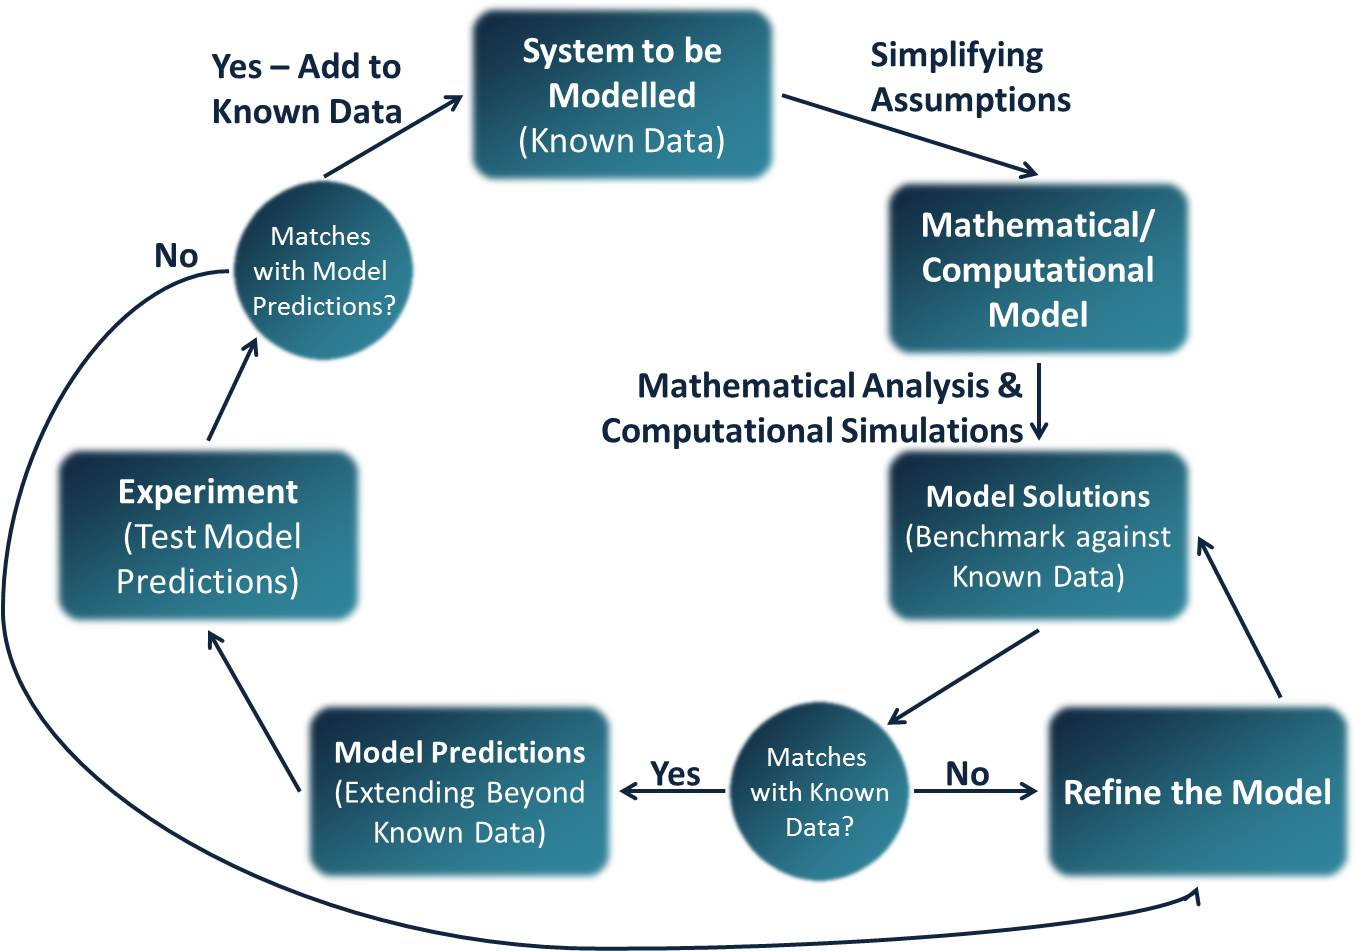
\includegraphics[width=1\linewidth]{ModellingCycle}
  \caption{Modelling cycle of the design of an \textit{in silico} model. Reproduced, with permission, from Roberts et al~\cite{Roberts_2016}.}
  \label{fig:ModellingCycle}
\end{figure}


Broadly speaking, a mathematical or \textit{in silico} model describes the state of a biological system using a set of dependent variables and the system of equations or rules which governs them.
\textit{In silico} simulations consist in solving the equations to find the dependent variables as functions of the independent variables.
Typical independent variables are time and space, but other choices are possible depending on the model.
When designing an \textit{in silico} model, one has to make choices among the variety of model types available.
This choice is informed by the system to be modelled, the question to be answered and the resources available (e.g., data or computational resources).
Because biological systems are so complex, the mechanisms modelled need to be kept to a minimum in order for the simulations to be tractable and interpretable.
The process of designing and refining an \textit{in silico} model follows a logic similar to experimental sciences and is summarised in Figure~\ref{fig:ModellingCycle}.
In this section, we give a brief overview of different model types that can be used to model the retina and typical challenges emerging when modelling biological systems.
A more comprehensive overview can be found in the work of Roberts et al~\cite{Roberts_2016}.

\subsection{Mechanistic vs phenomenological models}

To model a biological system, a relationship between the variables is hypothesised.
For all types of model, the hypothesised relationship needs to be validated against data and reviewed accordingly (see Figure~\ref{fig:ModellingCycle}).
In phenomenological models, a relationship that best describes the data is used, without reference to the processes underlying the observed phenomenon.
Curve fitting models, such as linear regressions, are examples of phenomenological models.
Conversely, mechanistic models incorporate into the model the biological processes that are thought to be underlying the observed phenomenon.
Those biological processes can, for the most part, be described using well-established physical laws, such as Fick's laws of diffusion.
For overly complex or unknown processes, a phenomenological description may be used within a mechanistic model.
Because simplifications are inherent to modelling, no model is fully mechanistic. % every mechanistic model eventually reduces to a phenomenological model.

\subsection{Model parameters}
All models involve a number of parameters.
Some of those parameters may be known, either from direct measurements or theoretical formulae.
Because a mechanistic model is physics-based, its parameters have a physical or biological definition whereas the parameters in a phenomenological model may not.
A direct consequence of this is that parameters in phenomenological models may be model specific and therefore cannot be used in a different model.

In cases where parameters are unknown, e.g., because they cannot be measured, \textit{in silico} models can provide estimates of the physical quantity by fitting parameters to data, when available.
Otherwise, analysis of the model predictions may still provide useful insights on the system's behaviour.
Indeed, in either case, tools such as sensitivity analysis and bifurcation analysis can provide insights on the system's behaviour for different parameter regimes.


\subsection{Initial and boundary conditions}

While initial conditions are the state of the system at time $t=0$, boundary conditions define the behaviour of the system at the boundaries of a spatial domain.
Classical boundary conditions may set the value of the dependent variables and are referred to as Dirichlet boundary conditions.
Alternatively, Neumann boundary conditions specify the spatial gradients of dependent variables at a boundary.
Finally, a condition on the sum of an independent variable's spatial gradient and value forms a Robin boundary condition.
For a system of differential equations to be well-defined and solvable, boundary conditions need to be specified.
%The number of conditions necessary depends on the order of the derivatives in the equations.

\subsection{Deterministic and stochastic models, continuum and discrete models}

When random events are left out of a model, two simulations will yield the same results, provided the parameters are left unchanged.
This kind of model is referred to as deterministic.
By comparison, stochastic models include a probabilistic component, e.g. the random movement of cells, which yields a different solution for each simulation.
Stochastic descriptions are often used for discrete models, e.g., agent-based models.
Discrete models simulate the behaviour of individual entities, such as cells, based on a set of pre-defined rules.
In contrast, continuum models assume the quantities of interest (e.g., number of cells) to be continuous variables with an infinite number of values between two points (e.g., cell concentrations).
% While the variables of a discrete model can be counted, continuous variables are measurable.
While discrete models can incorporate more details, continuum models allow for rigorous mathematical analysis.
A further limitation of discrete models includes the drastic increase in computation times as the number of objects simulated increases.

\subsection{Differential equations}

Many models describe the spatial and temporal behaviour of a quantity within a biological system using differential equations.
Differential equations relate one or more unknown dependent variables with their derivatives. 
Derivatives represent the rate of change of a dependent variable with respect to changes of an independent variable (e.g., the slope of a curve at a given point is the derivative of the dependent variable with respect to the independent variable).
If the equation involves derivatives of a single independent variable, it is referred to as an ordinary differential equation (ODE).
Otherwise, if more than one independent variable is involved in the derivatives, it is referred to as a partial differential equation (PDE).

Differential equations are mathematically tractable - namely, analysis tools can be rigorously applied to the analysis of the model.
Differential equations can be solved analytically, where the solution can be given as an algebraic function, or numerically, where an approximate solution is found for a pre-specified finite number of values of the independent variables.

PDEs often arise when the spatial distribution of the quantity of interest is needed.
However, the spatial aspect is not always relevant to the research question being investigated.
In such cases, an ODE relating a function and its time derivative can be used.
ODEs can also be used to model a system along a single spatial dimension at steady state, defined below.

Assuming a steady state is a common simplifying assumption that helps reduce the complexity and increase the interpretability of the system by ridding the model of the time component.
This reduction follows from assuming that the system, when not perturbed, does not change over time, hence the time derivative of the functions describing it are zero.
Similarly, spatial derivatives can be suppressed by assuming that the quantity is homogeneously distributed throughout space, an assumption termed well-mixed.
A well-mixed assumption may be used in some cases to justify the use of a compartmental model.

Compartmental models describe a system as separated compartments that can interact with each other, e.g., drug concentration in the eye can be described by vitreal, retinal and choroidal compartments, with mass exchange between adjacent compartments.
Lumped parameter models are a special case of compartment models, where numerous connected systems (e.g., blood vessels) are treated as a single entity, with the contributions of individual objects being lumped into parameters.
For instance, when modelling blood flow in a network of vessels, one may aggregate arterioles, capillaries and venules in separate compartments.
The properties of individual vessels are lumped into parameters that encompass the properties of the compartments (e.g., vascular resistance, oxygen extraction, storage capacity).
Compartmental models describe the system with a set of ODEs for each of the compartments or entities.

Systems of ODEs are typically simpler to solve, both analytically (by hand) and numerically (on a computer), and to mathematically analyse compared to PDEs.
The possibly complex geometry of biological systems may prove to be a challenge in the analysis of PDEs.
Approximating the geometry with simpler shapes such as spheres and rectangles, may allow derivation of analytical solutions or, at least, greatly reduce the time needed to numerically solve the equations.

Numerically, differential equations are solved by discretising the space and time variables into a mesh (that is, reducing the continuous variables to a finite number of points).
Solutions are calculated at the nodes of the mesh by solving a matrix equation (system of linear/non-linear algebraic equations).
The size of the matrix depends on the refinement of the mesh, with denser meshes yielding larger matrices.
Therefore, mesh size provides some degree of control over the computational complexity of the model - that is the time and memory needed to run a simulation.

Nonetheless, systems which span multiple spatial or temporal scales, which often arise in biology, can be computationally challenging to solve.
Indeed, smaller scales enforce smaller mesh sizes in order to account for the refined details of the geometry or of the mechanisms working on different time scales.
This issue appears, for example, when modelling the delivery of oxygen from retinal capillaries to a slab of tissue.
While the size of the tissue may be of the order of millimetres, the numerous blood vessels are, in contrast, of the order of micrometres, hence enforcing a mesh size of the order of micrometres.

In problems where separate mechanisms interact with each other (e.g., oxygen transport in the capillaries and oxygen diffusion in the tissue), the value of one dependent variable may depend upon that of other dependent variables.
The model is then said to be coupled.
While coupling and multiple scale in a model add to the difficulty of solving the equations, various mathematical techniques may help in reducing the complexity (e.g., homogeneneisation methods, multiple-scale analysis).
However, those tricks are often problem-specific and hard to generalise.

In addition, the often nonlinear behaviour of biological processes can affect the computational cost of running simulations.
Indeed, solving nonlinear equations most often requires solving a series of subproblems until the difference between successive iterations becomes small enough.

When complex nonlinearities are combined with multiple scales, the time required to solve a set of equations increases dramatically.
For these reasons, computation time remains a barrier to the use of \textit{in silico} models for real-time simulations in the clinic.
However, computational power is continuously increasing and it is only a matter of time until complex \textit{in silico} models can be used for real-time decision making.





\section{Retinal haemodynamics, vascular diseases, neovascular age-related macular degeneration and diabetic retinopathy}\label{sec:RetinalHaemodynamicsNAMDDR}

Adequate blood flow is essential for the supply of nutrients and removal of cellular waste required to maintain visual functions.
The atypical dual circulation of the retina is both complex and fragile.
It is thought that the inner vessels perfuse the inner \SIrange{60}{80}{\percent} of the retina, while the choroid supplies the remaining more metabolically active outer layers around the photoreceptors~\cite{Birol_2007}.
It is also known that ocular blood flow is affected by, among other things, IOP, systemic blood pressure, metabolic activity and oxygen saturation of the blood~\cite{Birol_2007,McCullough_1997,Palkovits_2014,Polska_2007,Pournaras_2008,Riva_1997,Wang_2014}.
Many retinal diseases have been linked, whether directly or indirectly, with abnormal haemodynamics~\cite{Hayreh_2004,Medina_2016}.
In fact, in certain diseases such as nAMD and DR, the blood supply is so disrupted that pathological neovasculature starts invading the retina.

One of the consequences of diabetes is the degeneration of the microvessels, such as capillaries, in the retina.
Eyes with DR see an increase in vascular permeability, a loss of the pericytes coating capillary walls, a thickening of the endothelial basement membrane abut to endothelial cells and a rarefaction of capillaries around the foveal avascular zone ~\cite{Medina_2016}.
These microvascular degenerations may cause microvascular occlusions, haemorrhages and oedema as well as macular ischaemia and consequent neovascular growth~\cite{Medina_2016}.

Haemorrhages, oedema, scarring and RPE or retinal detachment are characteristics of nAMD associated with macular neovasculature~\cite{Gupta_2015,Jager_2008}.
Similarly to DR, neovasculature in nAMD is believed to be a result of an upregulation of VEGF by RPE cells~\cite{Jager_2008}.
However, the pathogenesis of nAMD remains unclear.
Dysfunctions of the retinal circulations and subsequent ischaemia could partly explain increased VEGF concentrations, though dysfunction of the RPE and Bruch's membrane have also been suggested as actors in the pathogenesis of nAMD~\cite{Ambati_and_Fowler_2012,Pemp_2008,Liu_1995}.

Besides DR, a number of conditions may cause blood vessels in the retina to clog or collapse.
Accumulation of plaque caused by, for example, cholesterol, or a blood clot (embolus) in blood vessels form an obstruction to blood flow~\cite{Medina_2016}.
Sickle cell retinopathy causes a stiffening of red blood cells which can also result in occlusion of arterioles or capillaries, but also of the CRA~\cite{Medina_2016}.
Mechanical pressures such as ocular hypertension can cause the collapse of veins, including the CRV, when the external pressure becomes higher than blood pressure~\cite{Hayreh_2004}.
Stiffening of the CRA is suspected to also compress the CRV~\cite{Medina_2016}.
Occlusion of arteries causes non-perfusion areas in the retina, stopping visual functions in the affected areas.
Irreversible damage to the retina starts appearing after \SI{100}{\min} of non-perfusion~\cite{Hayreh_2004}.
Other symptoms include retinal oedema and, in some cases, neovascularisation in various locations, including the optic disc and the retina~\cite{Medina_2016}.

In proliferative DR and nAMD, haemorrhages, oedema, scarring and ischaemia cause a rapid degeneration of the photorectors and the RPE and subsequent loss of sight~\cite{Gupta_2015,Jager_2008,Roberts_2020, Waldstein_2016}
These are consequences of the growth of leaky blood vessels, referred to as neovasculature, in the neural retina, especially in the macula.
Pathological angiogenesis is driven by gradients of VEGF.
Binding of free VEGF molecules to receptors on the walls of existing blood vessels triggers the proliferation and migration of endothelial cells along those gradients~\cite{Ferrara_2004}.
To prevent or halt complications due to neovasculature, clinicians often resort to anti-VEGF drugs which bind to free VEGF molecules to prevent their binding to the vasculature.

Glaucoma is thought to be a result of a combination of ocular hypertension and changes in cerebrospinal fluid pressure and retinal blood pressure which creates a pressure gradient around the optic nerve~\cite{Band_2009,Nickells_2012}.
The increased mechanical stress on the tissue induced by these changes causes a degeneration of the ganglion cell bodies (in the GCL, see Figure~\ref{fig:architecture-eye}) and axons (forming the optic nerve).
Vision loss in glaucoma is due to the loss of connectivity between the retina and the brain and cannot be recovered~\cite{Quigley_2011}.


In this section, we review \textit{in silico} models that contribute to our understanding of the normal physiology of the retina as well as models aiming at deciphering the aetiology of various diseases which may be linked with haemodynamics in the retina and the underlying choroid.
More comprehensive reviews of models of the microcirculation, angiogenesis and oxygen delivery can be found in the work of Arciero et al~\cite{Arciero_2019, Arciero_2017}.
In addition, we present models of the pharmacokinetics (PK) and pharmacodynamics (PD) of anti-VEGF treatment.


\subsection{Retinal haemodynamics} \label{subsec:RetinalHaemodynamics}

\begin{figure}[t!]
  \centering
  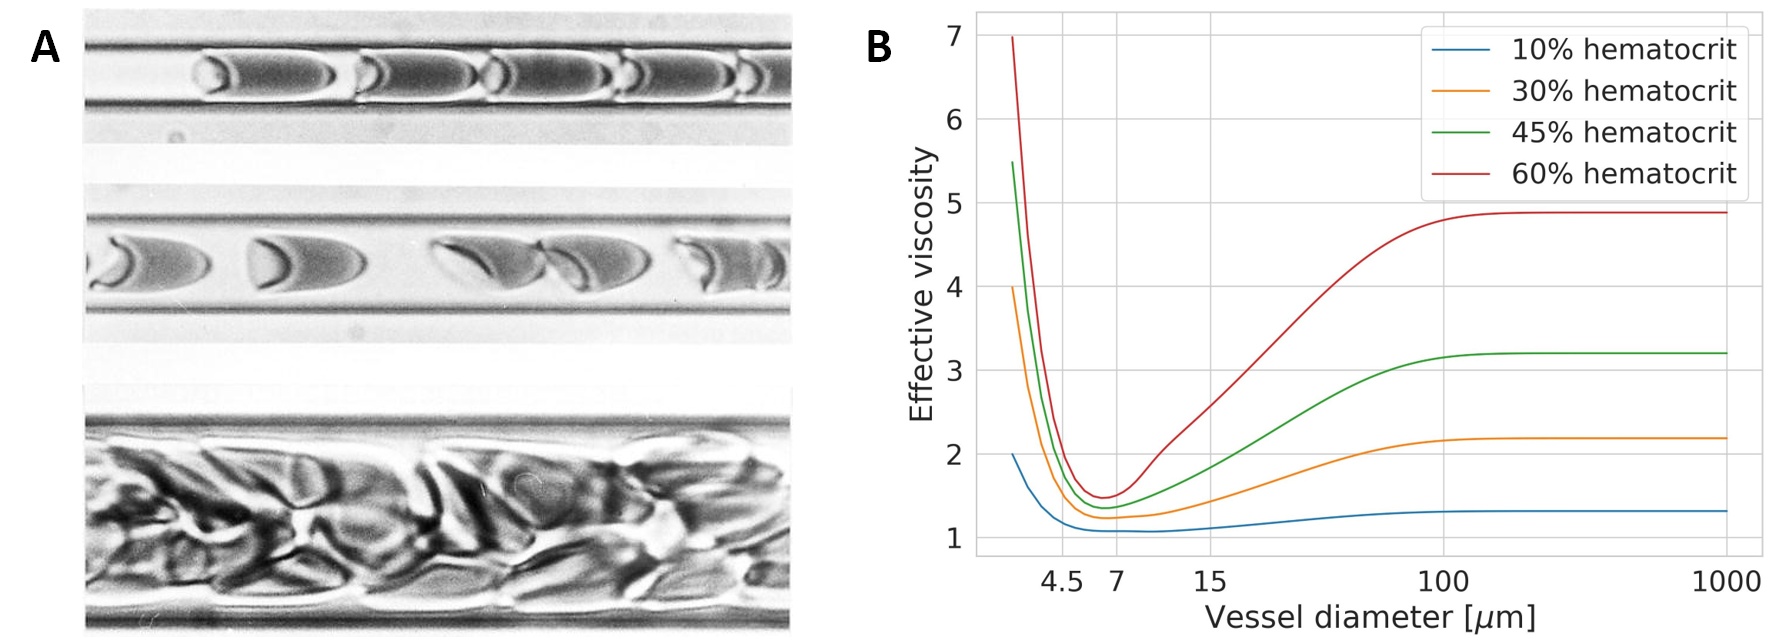
\includegraphics[width=1\textwidth]{EffectiveViscosity}
  \caption{Example of the effect of capillary calibre on the flow of blood. (\textbf{A}) Red blood cells in suspension in blood flowing within tubes of different diameters: \SI{4.5}{\micro\meter} (top), \SI{7}{\micro\meter} (middle) and \SI{15}{\micro\meter} (bottom). One can observe the flow of cells converging into a single file, surrounded by a layer of plasma as the diameter moves from \SI{15}{\micro\meter} to \SI{7}{\micro\meter}. A cell's shape adapts to fit into the tube as the diameter approaches that of the cell (top row). Reproduced, with permission, from Secomb~\cite{Secomb_2003}. (\textbf{B}) Example of an empirical law for the effective viscosity of blood accounting for the F\r{a}hr\ae us-Lindqvist effect, a description of the decrease in blood viscosity with vessel diameter, and increased vascular resistance in smaller capillaries from the work of Secomb and Pries~\cite{Secomb_2013}. Note that the effective viscosity depends on the blood's concentration in red blood cells (hematocrit).}
  \label{fig:effectiveViscosity}
\end{figure}

Retinal haemodynamics models are concerned with describing blood flow within the inner retinal or choroidal circulations and often rely on the Hagen-Poiseuille equation to determine flow in vascular segments.
This equation is a simplification of the more comprehensive Navier-Stokes equations and is derived by making a number of assumptions (see \textit{Additional information}).
The Hagen-Poiseuille equation states that blood flow velocity ($Q$) in a vessel of length $l$ and radius $r$ is driven by a pressure drop ($\Delta p$) according to:
\begin{equation*}
  \label{eq:Hagen-Poiseuille}
  Q = \mathit R\times\Delta p \mbox{, where } \mathit{R} = \frac{8\mu l}{\pi r^4},
\end{equation*}
where $\mu$ is the apparent viscosity of blood which may account for changes in vascular resistance ($\mathit R$) in vessels of varying diameter (see \textit{Additional information} and Figure~\ref{fig:effectiveViscosity}).
The fourth power of the radius in the formulation of vascular resistance describes the strong effect that even small contractions or dilations of a vessel can have on blood flow.
This relation between radius and flow is at the source of the autoregulation ability of blood vessels, which adapt their radius in response to a number of different cues~\cite{Kur_2012}.
The cellular constitution of retinal vessels suggests that blood flow is mainly regulated by arteries and arterioles~\cite{An_2020,Kur_2012}.
Evidence suggests that the choroid is also able, maybe to a lesser degree, to regulate blood flow~\cite{Polska_2007,Riva_1997}.
Neurological regulation (regulation by the autonomic nervous system) of choroidal blood flow has been suggested, in view of the rich innervation of choroidal vessels~\cite{BeharCohen_2020,Polska_2007}.

\textit{In silico} models provide valuable insights into the mechanisms that combine to provide healthy perfusion or, conversely, create conditions for the onset of retinal pathologies.
The assumptions made in these models can be validated by comparing simulation results with \textit{in vivo} measurements of changes in blood flow or vessel radii.
Vessel radius in the inner retina can be measured from retinal scans such as fundus photographs, fluorescein angiograms or OCT angiograms.
Blood flow can be measured using devices such as a Doppler flowmeter or Doppler Fourier-domain OCT, in combination with radius measurements~\cite{DoblhoffDier_2014,Wang_2009}.
The blood oxygen saturation can also be measured \textit{in vivo}~\cite{Geirsdottir_2013}.
Reliable measurement of blood flow or vessel radii in the choroid is more difficult, though changes in haemodynamics can be observed \textit{in vivo}~\cite{Riva_1997,Scherm_2019}.

\begin{tcolorbox}[title=Additional information -- Fluid flow modelling]
  \begin{itemize}
  \item Viscous fluids such as blood are modelled by a set of differential equations --- the Navier-Stokes equations --- relating the acceleration, velocity, convection, density and pressure of a fluid.
    Solving those equations can be problematic in complex geometries, for example, in a large network of vessels.
  \item Those equations simplify to the Hagen-Poiseuille equation (see main text) when assuming that the fluid is Newtonian and the flow incompressible and laminar.
    The Hagen-Poiseuille equation is relatively simple to solve, even on large vascular networks.
  \item An incompressible fluid has a constant density regardless of the pressure, while the fluid isotropic if its properties are the same in all directions.
  \item A Newtonian fluid is one with a constant viscosity for given pressure and temperature, regardless of the amount of shear (the stress arising from the friction of fluid particles) it is subject to.
  \item A Newtonian fluid flowing within a pipe is called laminar when fluid particles (e.g., red blood cells, blood plasma) move along smooth paths with no mixing between each path.
    This kind of flow is opposed to turbulent flow, which appears when the velocity of the flow exceeds a threshold determined by a combination of the fluid's viscosity and density and the pipe's dimensions.
  \item The propensity of a fluid to flow in laminar or turbulent fashion is summarised by the dimensionless (without physical units) Reynolds number. This number is the ratio of inertial forces to viscous forces.
  \item Laminar flows show a parabolic velocity profile across the pipe (or vessel) cross section, with peak velocity at the centre and null velocity at the walls.
  \item As demonstrated by F\r ahraeus and Lindqvist, viscosity decreases with vessel width as red blood cells align into a single file, as illustrated in Figure~\ref{fig:effectiveViscosity}\cite{Faahraeus_1931}.
  \item Empirical viscosity laws are used to account for the so-called F\r ahraeus-Lindqvist effect and the dramatic increase in vascular resistance seen in capillaries smaller than red blood cells, an example of which is shown in Figure~\ref{fig:effectiveViscosity}~\cite{Haynes_1960,Pries_1990,Secomb_2013}.
  \end{itemize}
\end{tcolorbox}


\subsubsection{In health}

Current understanding of perfusion in the retina has advanced significantly in recent decades.
Inner retinal haemodynamics in particular have been studied extensively due to the relative ease of imaging this vasculature with OCT and fundus photography.
Conversely, outer retinal haemodynamics (perfused by the choroidal circulation) are less well understood due to the difficulty in imaging these vessels.
Below we review models that simulate perfusion and oxygen transport in healthy retinas.

\begin{figure}[t!]
  \centering
  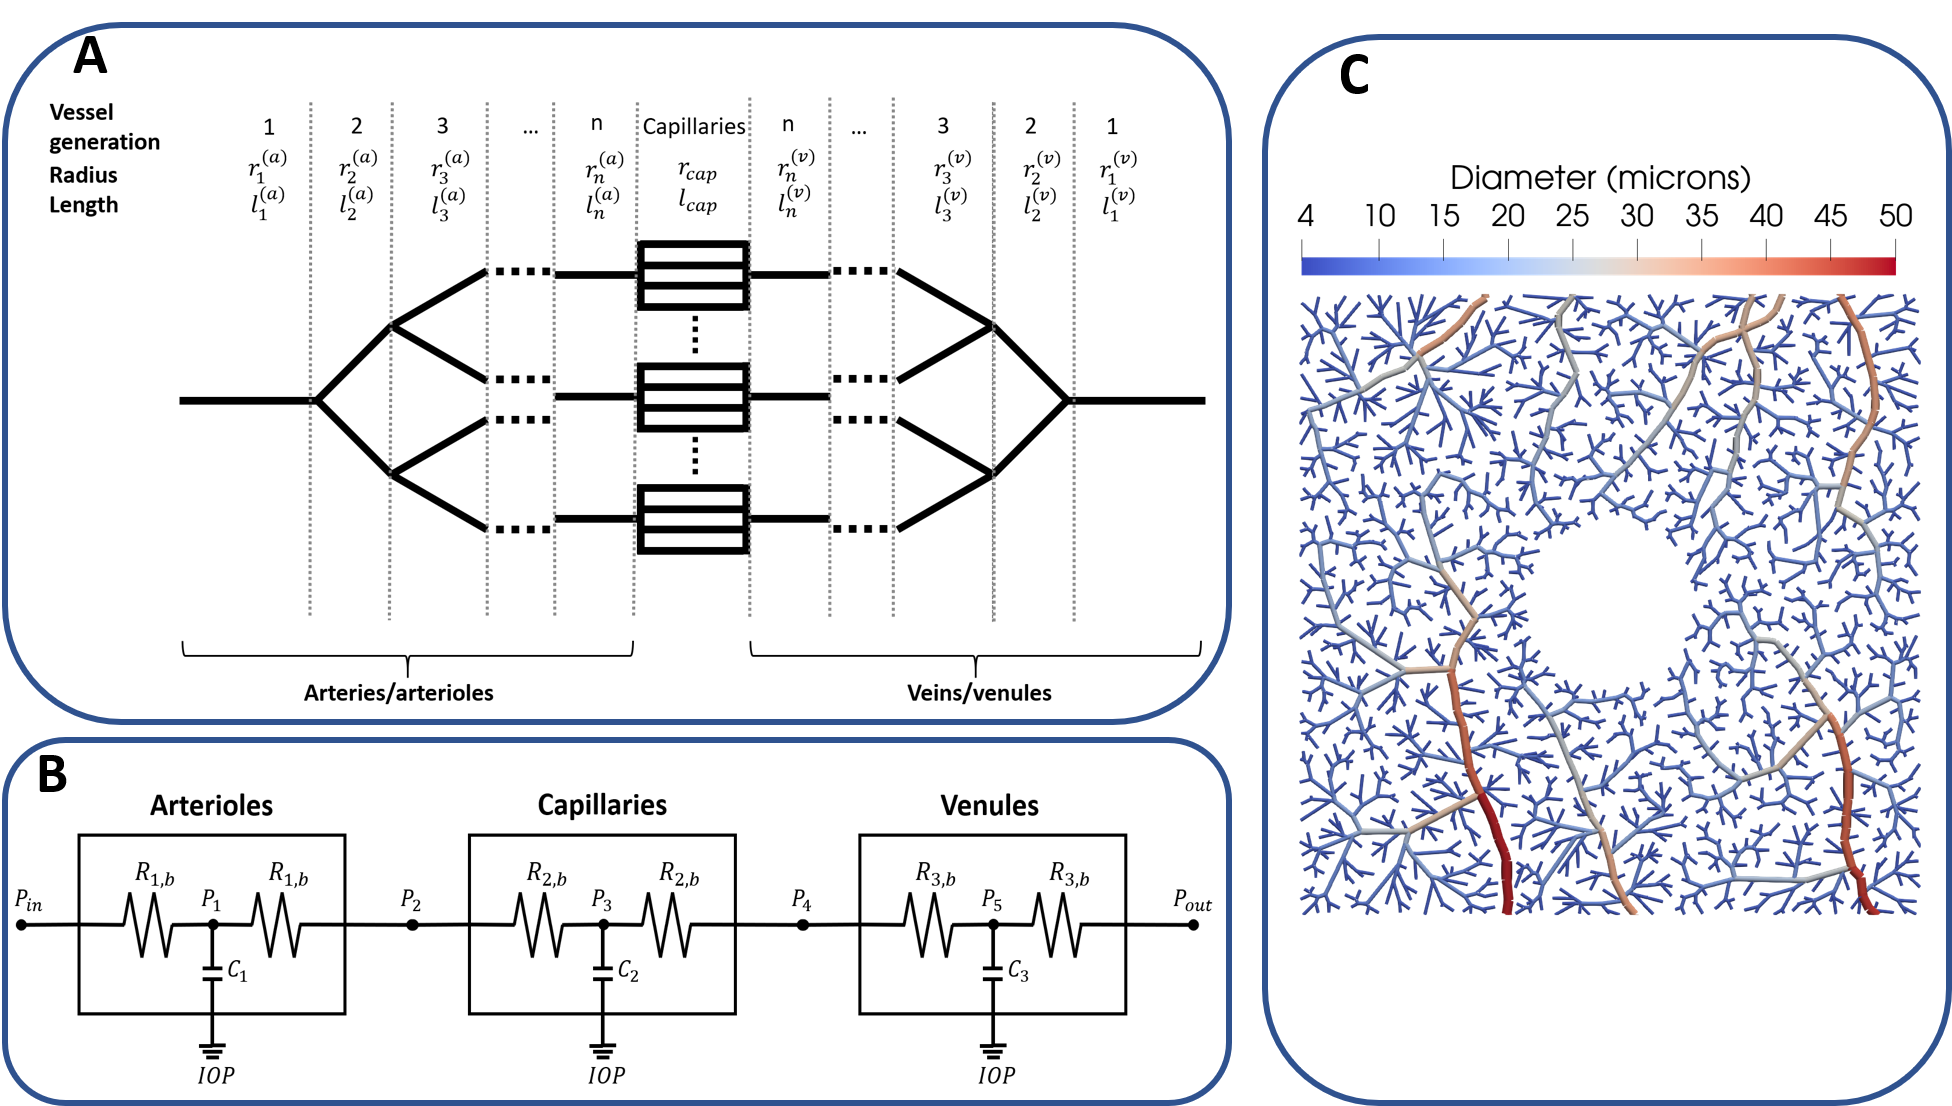
\includegraphics[width=\textwidth]{NetworkModels}
  \caption{Different representations of the microvasculature in haemodynamics models. (\textbf A) An example of a dichotomous, symmetrical branching network similar to Takahashi et al.'s network~\cite{Takahashi_2009}. The radius of branching vessels follows Murray's law, namely, $r_1^\gamma = r_2^\gamma+r_3^\gamma$ where $r_1$ is the radius of the parent vessel, $r_1,r_2$ are the radii of the branching vessels and $\gamma$ is an exponent translating the fractal aspect of the vasculature. (\textbf{B}) An example of lumped parameter model where characteristics of the arterioles, capillaries and venules are summarized by resistance ($R_i$) and capacitance ($C_i$) parameters which may vary due to the action of external factors (e.g., changes in IOP (IOP)). Blood pressure ($P_i$) is defined at given nodes within and between vascular compartments. (\textbf{C}) An example of an artificial, realistic microvascular network of the macula generated by a constructive constraint optimization algorithm~\cite{Talou_2021}.}
  \label{fig:NetworkModels}
\end{figure}

\paragraph*{Haemodynamics in artificial retinal vasculature}

Takahashi et al. proposed an arterio-venous dichotomously branching and symmetric network in which all vessels within a given generation are identical~\cite{Takahashi_2009}.
The diameter of the branching vessels follows the principle of least energy described by Murray's law, stated in Figure~\ref{fig:NetworkModels}~\cite{Murray_1926}.
This theoretical model was used to describe the distribution of flow and other haemodynamic parameters across the normal retinal vasculature.
While clinical studies often report changes in the diameter of large retinal vessels in various conditions, its relationship with total retinal blood flow, a clinically relevant parameter, is unclear.
Takahashi et al.'s network has been adapted to further investigate the physiology of the retinal vessels, in conjunction with clinical experiments~\cite{Aschinger_2017,Pappelis_2020}.
One of these studies showed that dilation of larger retinal vessels do not necessarily induce a change in total retinal blood flow~\cite{Aschinger_2017}.
In fact, simulations of different vasodilation patterns suggested that the diameter of smaller vessels, which elude measurements, was the main determinant of blood flow~\cite{Aschinger_2017}.
However, the validity of the modelling assumption that capillaries are able to vary their diameter remains unclear~\cite{Kur_2012}.
Pappelis et al. used clinical information to create patient specific networks based on Takahashi et al.'s method~\cite{Pappelis_2020}.
The model includes an autoregulation component as a function of retinal perfusion pressure (pressure entering the CRA, estimated as the difference between systemic blood pressure and IOP) and predicted the blood flow response to increases in IOP or drops in retinal perfusion pressure.
This allowed prediction of the autoregulation capacities of retinas in patients treated for hypertension or in eyes subject to ocular hypertension.
It showed that the retinas of both healthy and hypertensive patients were closer to the lower limit of autoregulation, suggesting that the retina may be more sensitive to decreases than to increases in perfusion~\cite{Pappelis_2020}.


\paragraph*{Effects of extravascular pressure on haemodynamics} %NOTE: this could be one section with the next one (Autoregulation pathways)

Lumped parameter models have been used to investigate the relationships between intravascular and extravascular pressures and haemodynamics in the retina and choroid~\cite{Chiaravalli_2021,Fawzi_2019,Guidoboni_2014a,Nelson_2017,Petersen_2022,Prudhomme_2021,Sala_2020,Salerni_2019}.
In these models, similar vessels are sorted into compartments, e.g., CRA, arterioles, capillaries, venules, CRV and choroid (see Figure~\ref{fig:NetworkModels}).
The physical processes within compartments and the interactions between them are summarized by a small set of parameters.
By analogy with electrical circuits, the haemodynamics in each compartment are characterised by a resistance (the combined effect of the vascular resistance of a compartment's vessels) and a capacitance (the total amount of blood that can be stored in the same vessels).

Lumped parameter models have been used to investigate the links between gravity-induced shifts in intracranial fluids, ocular fluids and pressures, and the loss of sight observed in astronauts~\cite{Nelson_2017,Petersen_2022,Salerni_2019}.
Nelson et al. proposed a baseline model simulating increases in ocular pressures secondary to such fluid shifts~\cite{Nelson_2017}.
The simplistic model predicted relatively well the response of IOP to changes in the gravitational environment or tilt of the body~\cite{Nelson_2017,Petersen_2022}.
A more comprehensive model including interacting brain, body and eye compartments showed that the retinal circulation was relatively spared from hypoperfusion compared to the choroidal circulation in microgravity conditions~\cite{Salerni_2019}.
\textit{In silico} models are particularly useful when scarcity of subjects (e.g., astronauts) and difficulty to reproduce the environment (e.g., long periods in microgravity conditions) hinder experimental research since they necessitate relatively little data.

\paragraph*{Autoregulation pathways}

Several lumped parameter models have been developed to better understand the mechanisms behind autoregulation in physiological conditions~\cite{Arciero_2008,Arciero_2013,Guidoboni_2014a}.
Arciero et al. developed two models using symmetric networks similar to Takahashi et al.'s to understand the information pathways leading to blood flow autoregulation in the retina~\cite{Arciero_2008,Arciero_2013}.
Both models assumed that only arterioles possess the ability to contract and dilate to regulate flow.
These models were used to investigate the response of individual and combined autoregulation pathways to changes in perfusion pressure or oxygen consumption rate of the cells.
Arciero's first model investigated the hypothesis that arterioles can contract in response to the oxygen saturation of blood in the downstream venules~\cite{Arciero_2008}.
The study showed that this autoregulatory pathways could account for the experimentally observed response of perfusion to changes in consumption rates.
This mechanism, along with responses to shear stress on the vessel walls and carbon dioxide concentrations, were modelled together in a subsequent study by Arciero~\cite{Arciero_2013}.
The study assessed each pathway's contribution to retinal perfusion.
The results showed that the response of arterioles to carbon dioxide concentration in the surrounding tissue and oxygen saturation in the venules was essential to retinal autoregulation~\cite{Arciero_2013}.

Guidoboni et al. considered the interplay between IOP, retinal haemodynamics, systemic blood pressure and autoregulation~\cite{Guidoboni_2014a}.
Instead of the mechanistic description of autoregulation proposed by Arciero et al., they used an empirical response function of arteriole diameter to changes in perfusion pressure.
% Another difference with previous work is the assumed capacity of the venules and central retinal vessels to dilate or collapse passively and, to some limited extent, in response to pressure gradients across their walls.
The retinal haemodynamics of six types of physiology (high, normal or low blood pressure, with or without working retinal autoregulation) were simulated across a range of IOP.
The model predicts the ranges of IOP within which each physiology can maintain relatively constant blood flow.
Experimental studies to elucidate the relationship between IOP and retinal haemodynamics by artificially elevating or lowering IOP reached inconsistent conclusions\cite{Conway_2010,Findl_1997}.
The dependence of these ranges to systemic blood pressure and autoregulation capacity, in combination with the small sample size in these studies may explain those inconsistencies~\cite{Guidoboni_2014a}.

\paragraph*{Oxygen transport and spatial models}

The transport and delivery of oxygen to retinal tissue has been modelled by several groups~\cite{Aquah_et_al_2021,Causin_2015,Liu_2009}.
The earliest model used a short arteriolar tree, taken from a retinal photograph of a healthy young volunteer, and solved the Navier-Stokes equations to obtain the haemodynamics in these vessels~\cite{Liu_2009}.
The downstream vasculature was represented as a structured tree extending the outlets of the segmented arterioles.
This model reproduced the distribution of intravascular oxygen observed \textit{in vivo} and could serve as a baseline to analyse oxygen distribution in realistic vascular networks.
However, reproduction of the retinal vasculature is limited to larger vessels.
Therefore, the use of artificial vasculatures (such as the one displayed in Figure~\ref{fig:NetworkModels}) with similar topological characteristics as the retinal vasculature may be useful to model the whole extent of the retinal vasculature.

Causin et al. used the fractal similarity between retinal vessels and diffusion-limited aggregation processes to generate a three dimensional network of three of the vascular plexi of the retina~\cite{Causin_2015}.
Oxygen transport throughout the extensive vascular network was modelled as well as the oxygen delivery to the tissue (modelled as a rectangular slab).
The good agreement with data validated the use of the artificial networks.
The effects of haemodynamic parameters on different parts of the tissue and the vasculature were analysed, demonstrating, among other things, the sensitivity of retinal ganglion cell layer perfusion to blood viscosity and metabolic consumption~\cite{Causin_2015}.

Several other studies have used vessels reproduced from images to analyse the distribution of blood flow and the influence of the morphology~\cite{Malek_2014,Malek_2015,Rebhan_2019}.
The use of realistic vascular networks provides a link between haemodynamics and clinically relevant indices.
The effect of tortuosity has been investigated on short, segmented sections of the retinal veins~\cite{Malek_2014}.
Malek et al. tried to characterise the flow distribution in reproduced arterioles and veins to quantify the impact of vessel tortuosity (a measure of how much a vessel differs from a straight line) on haemodynamic parameters~\cite{Malek_2014,Malek_2015}.
The Navier-Stokes equations are used to find flow within the arterioles, while peripheral circulation is accounted for by an impedance condition at the outlets of the segmented tree.
The deformation of vessels caused by the pulse of blood is a computationally complex task to model and a simplified model has been developed and applied to a similar reproduction of the retinal vasculature, with a brief analysis of its effects on haemodynamics~\cite{Aletti_2016}.
Notably, Rebhan et al. have considered the interactions of retinal haemodynamics and tissue stress using reproductions of the large vessels of healthy and diseased eyes, an aspect previously overlooked that may have importance in, e.g., glaucoma and diabetes~\cite{Rebhan_2019}.

%%% COULD BE DELETED?
\textit{In silico} models have also been developed to understand how the retinal vasculature develops.
Some of these models have been reviewed previously~\cite{Arciero_2019,Roberts_2016}.
However, the role of haemodynamics in angiogenesis of the vascular beds is still elusive.
Bernabeu et al. proposed a model of blood flow in a reconstructed murine vasculature that can be used to simulate the haemodynamics forces that cannot be measured in small capillaries but may affect angiogenesis~\cite{Bernabeu_2014}.
Others looked at how the branching patterns in the early development of the murine retina may affect later development~\cite{Mirzapour_Shafiyi_2021}.
The results showed that hyper-branching behaviours in the young vascular bed reduces the blood supply, and hence the oxygen, at the growing ends of the vasculature.
The lack of oxygen on this front may drive up-regulation of vascular growth factors promoting vascular growth.


\paragraph*{Haemodynamics in the central retinal vessels}

Others have used finite element modelling, a technique suitable for modelling of mechanistic forces, to understand the blood flow in the central retinal vessels~\cite{Guidoboni_2014,Jin_2020}.
The central retinal vessels enter the retina along the optic nerve where they are under pressure from the surrounding tissue, the cerebrospinal fluid surrounding the eye, the IOP and, potentially, the artery and vein may also compress each other~\cite{Nickells_2012}.
The lamina cribrosa's purpose is to act as a buffer protecting the vessels where the pressures described above interact.
Guidoboni et al. simulated the displacement of the lamina cribrosa and the stress due to changes in IOP and pressure induced by the cerebrospinal fluid~\cite{Guidoboni_2014}.
The simulation of blood flow in the CRA showed good agreement with measurements made during IOP elevation, suggesting that the observed decrease in blood flow velocity is caused by the lamina cribrosa compressing the artery.
Note that this model assumed a constant blood pressure, averaging the systolic and diastolic blood pressures.
Pulsatility may have a significant impact on IOP and, consequently, blood flow in the central retinal vessels and has been investigated within a more comprehensive model of the ocular structures~\cite{Jin_2020}.


Whether the vascular plexi in the retina, namely, the SVP, ICP and DCP, are connected \textit{in series} or \textit{in parallel} is still unclear.
The \textit{in parallel} configuration supposes that both arterial and venous connections exist between plexi.
Conversely, in the \textit{in series} configuration, blood inflow comes solely from the SVP, while venous drainage occurs only in the DCP.
We refer the reader to Figure 1 in the paper by Chiaravalli et al. for a schematic of these two configurations~\cite{Chiaravalli_2021}.
The lumped parameter models developed in this paper simulate haemodynamics between the CRA and the CRV in five vascular compartments~\cite{Chiaravalli_2021}.
The authors modelled both configurations and compared the responses of each plexi to IOP elevation and occlusion of the CRV.
The model showed that the \textit{in series} configuration better captured the response observed in clinical studies, and may better describe the actual physiology of the retinal vasculature.

\paragraph*{Choroidal circulation}
While the inner retinal vasculature feeds the inner third of the retina, the remaining two thirds are perfused by the choroidal circulation.
The CC (see Figure~\ref{fig:architecture-eye}) provides oxygen across BrM to the photoreceptors and other neuronal cells of the outer retina through diffusion only.
Therefore, a high vascularisation is necessary to provide enough oxygen despite the distance.
Defects in choroidal blood flow are associated with major retinopathies such as nAMD and DR~\cite{Pemp_2008}.
Despite its importance, little is known about the physiology of the choroid.
Likewise, little work has been done on modelling choroidal circulation.
Early work tried to decipher whether the choroid of rabbits was able to regulate its flow in response to changes in systemic pressure~\cite{Kiel_1992}.
Simulations in conjunction with experimental evidence suggests a autoregulatory reflex in the choroid triggered by blood pressure.
Since then, only Zouache et al. have modelled the physiology of the choroid and its peculiar architecture~\cite{Zouache_2015,Zouache_2016}.
By simulating the lobular structure of the CC, they investigated the effects of the geometry of lobules on the flow of blood.
Their work suggested that the distribution of flow separators in the CC and the location of inlet and outlets in individual lobules may explain the localisation of oedema or neovasculature in diseased eyes~\cite{Zouache_2015}.


\subsubsection{In disease}

%As mentionned previously, many retinal pathologies have or may have a link with irregular haemodynamics.
In disease, the haemodynamics of the retinal circulations may change drastically; however, the exact role of haemodynamics in the aetiology of vascular retinal diseases is still elusive.

\paragraph*{Models of pathological geometries} 

Rebhan et al. compared haemodynamics in a model of vascular networks segmented from a healthy eye and eyes affected by glaucoma or diabetes~\cite{Rebhan_2019}.
The embedding of vessels in tissue revealed an increase in wall shear stress in diseased eyes compared with the healthy one.
However, it was noted by Rebhan et al. that the absence of downstream vasculature is likely to affect the quality of predictions~\cite{Rebhan_2019}.
Along the same lines, higher vascular tortuosity, a common sign of aging and disease, has been shown computationally to increase the pressure drop across the vasculature~\cite{Malek_2014}.
However, vessel-tissue interactions were not considered in the model.

Eyes with visual impairments such as myopia see a progressive change of the shape of the retina and may develop neovasculature~\cite{Medina_2016}.
This suggests a link between the curvature of the eye and retinal perfusion.
However, the effects of curvature have been assumed insignificant in most haemodynamics models to date.
Dziubek et al. modelled this curvature by representing the retina as a thin, curved surface, within which an artificial network of vessels is embedded~\cite{Dziubek_2015}.
The tissue is considered a porous medium --- with the embedded vessels acting as pores --- with pressure in the tissue described by Darcy's law.
% Arteriolar, capillary and venular networks are kept virtually separated but communicate through a `hierarchical' velocity variable, as opposed to the spatial velocity which describes movement throughout the retinal surface.
The dichotomous tree proposed by Takahashi et al. was used to generate the vascular networks.
The model confirms clinical suspicions of a change in retinal haemodynamics due to ocular curvature.
Furthermore it highlighted the non-uniform effects on the retina, with the temporal region being less affected by ocular shape\cite{Dziubek_2015}.

\paragraph*{Models of glaucoma and vessel occlusion}

Numerous models have been developed to explain alterations of blood flow observed in eyes subject to glaucoma or vessel occlusion\cite{Chuangsuwanich_2016,Guidoboni_2014,Sala_2018,Sala_2020}.
Elevated IOP, a hallmark of glaucoma, is expected to affect the retinal circulation, causing loss of sight.
Modelling of the interactions between the ocular structure surrounding the central retinal vessels has shown the role of a stiffened lamina cribrosa resulting from such conditions~\cite{Guidoboni_2014}.
In addition, the model by Guidoboni et al. showed that the geometry of the sclera and the lamina cribrosa affect the sensitivity of blood flow to elevation of IOP.
This framework was extended in Sala's thesis to create the `Ocular Mathematical Virtual Simulator', a simulation environment for the interactions of haemodynamics and biomechanics in the eye~\cite{Sala_2018,Sala_2020}.
This environment allows haemodynamics simulations of individual patients characterised by a handful of parameters, yielding significantly different results for each combination of parameters.
Results showed that high IOP can cause collapse of the CRV and major differences in the displacement of the lamina cribrosa.
Interestingly, it showed that the perfusion of the lamina cribrosa is also negatively affected by ocular hypertension, a potentially significant mechanism in the understanding of glaucoma~\cite{Sala_2020}.
Perfusion and haemodynamics within the lamina cribrosa have been modelled separately using a large number of artificial capillary networks statistically representative of different morphologies of the lamina cribrosa~\cite{Chuangsuwanich_2016}.
For a review of the use mathematical models in glaucoma research, we refer the reader to the review by Harris et al~\cite{Harris_2013}.

\paragraph*{Models of diabetic retinopathy}

Microaneurysms are an early manifestation of DR where the walls of capillaries form outpouchings disrupting blood flow and rendering them susceptible to rupture.
We found four studies investigating haemodynamics in reconstructed microaneurysms using computational fluid dynamics models~\cite{Bernabeu_2018,Czaja_2022,Li_2020,Li_2022}.
Bernabeu et al. considered the shape of microaneurysms and how it influences haemodynamics, and in particular shear rates, in an attempt to determine predictors of the likelihood of leaking blood clotting~\cite{Bernabeu_2018}.
Similarly, Czaja et al. investigated wall shear stress in microaneurysms in the event of stiffened red blood cells, another symptom of diabetes~\cite{Czaja_2022}.
A notable difference with the previous model is the use of cell-resolved blood flow simulations, where individual cells are modelled and transported by blood flow.
This allowed separate investigation of red blood cell and platelet flows, demonstrating the differences in penetration through the microaneurysm between the two cell types.
Stiffened red blood cells were found to induce higher wall shear stress, both in the aneurysm sac and in the vessels feeding and draining it.
In two studies, Li et al. also simulated the flow of red blood cells and platelets in microaneurysms with a focus on platelet flow through the microaneurysm, as they may be linked with the formation of blood clots~\cite{Li_2020,Li_2022}.

Panretinal photocoagulation therapy is a common procedure to treat ischaemia in retinas with proliferative DR.
While practice has shown the efficiency of the procedure, its mechanisms of action remain unclear.
It is thought that the procedure acts by reducing the oxygen consumption of the photoreceptors affected by the laser-induced burn~\cite{Fawzi_2019,Gast_2016}.
However, effects of the therapy on blood flow have been observed~\cite{Fawzi_2019}.
With a simple lumped parameter model and the assumption that panretinal photocoagulation increases vascular resistance in the periphery of the macula, Fawzi et al. showed how the surgery could increase macular blood flow~\cite{Fawzi_2019}.
The increased perfusion in the macula would then explain the decrease in VEGF concentrations and the subsequent regression of neovasculature.
The model predictions are consistent with the seemingly increased flow in macular capillaries~\cite{Fawzi_2019}.
The burn patterns used in panretinal photocoagulation are also subject to debate.
Gast et al. investigated the effects of different patterns on the propagation of ischaemia due to capillary occlusion~\cite{Gast_2016}.
The model showed how different burn patterns affect the propagation of ischaemia and suggested that targeting the non-ischaemic peripheral retina with appropriate patterns may be effective at containing it.

\subsection{Anti-VEGF therapy in nAMD and DR}\label{sec:Anti-VEGF}

\begin{figure}[t!]
  \centering
  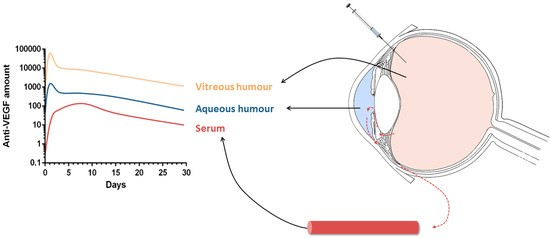
\includegraphics{AntiVEGF}
  \caption{Schematic of anti-VEGF concentration profiles in compartments of a compartmental pharmacokinetics model. Reproduced, with permission, from Garc\'ia-Quintanilla et al~\cite{GarciaQuintanilla_2019}.}
  \label{fig:AntiVEGF}
\end{figure}

The treatment of neovasculature in proliferative DR and nAMD takes the form of frequent injections of VEGF-inhibiting molecules that bind to the free VEGF present in the retina, ultimately inhibiting the angiogenic process.
Anti-VEGF drugs are injected directly in the vitreous humour though alternative delivery techniques are being investigated~\cite{Kim_2021}.

Molecules present in the vitreous are naturally eliminated through the aqueous humour flow, referred to as the anterior clearance route.
The posterior clearance route refers to clearance through the choroidal circulation.
In addition, the ILM and RPE, bounding the inner and outer retina respectively, act as barriers to the molecules~\cite{Park_2015}.
Therefore, the presence of the drug in the retina and choroid is limited to a fraction of the injected dose. 

Despite its general efficacy, current treatment strategies are sub-optimal for some patients in terms of dosage and intervals between injections.
Eyes showing little to no improvement in their condition are referred to as non-responsive and present a real challenge for clinicians.

Furthermore, VEGF induced angiogenesis is a natural response to inflammation and hypoxia, in the eye and the rest of the body. 
Therefore, repeated injections pose a number of problems.
Firstly, the intravitreal injections (IVI) can cause further inflammations within the retina, triggering additional VEGF upregulation~\cite{Iyer_2022}.
Secondly, with the current doses, the unbound anti-VEGF molecules that are cleared from the eye are found in significant levels in the systemic circulation, raising concerns about the safety of IVI.
Indeed, while it is still a matter of debate, it has been suggested that the IVI of anti-angiogenic molecules could be linked with serious adverse effects including haemorrhages and strokes~\cite{Avery_2016, Kaiser_2019, Maloney_2021}.
Knowledge of the total exposure of the retina and the CC to the drug is important to develop better therapeutic molecules and administration strategies and to reduce the risk and burden on the patient.

While aqueous and vitreous humours can be sampled \textit{in vivo}, the concentrations of drug in the retina and choroid remain unknown. 
Therefore, estimates of the retinal kinetics of molecules are often based on either animal experiments or on samples of the aqueous humour, the vitreous humour and systemic plasma.
Mechanistic PK and PD models can help overcome the issue of the lack of \textit{in vivo} data in the retina and provide insight into the complex relationships between drug characteristic and physiological parameters.
Those models simulate the concentration-time profiles of a molecule in the eye (see Figure~\ref{fig:AntiVEGF}) and can be validated by comparison with data sampled from the systemic circulation or ocular fluids.
This section is dedicated to computational models of VEGF and its inhibitors, both individually (PK models, VEGF production models) and combined (PD models).

\paragraph*{Compartmental PK/PD models}

Often in PK analysis of ocular or systemic fluid, the half-life of a molecule is estimated by fitting exponentially decaying curves to the data in order to compute the total exposure to the drug (area under the concentration-time curve) and maximal concentration~\cite{Bakri_2007, Kaiser_2019, Park_2015, Park_2016, Xu_2013}.
This assumes that the clearance rate of molecules in the eye is proportional to their concentration at all times and ignores potential effects of interactions with the tissue or the presence of multiple clearance pathways (e.g., the aqueous humour outflow and the choroid circulation).
Understanding the determinants of the PK of anti-VEGF molecules in the eye is essential to develop more effective molecules and such simple models do not provide this kind of insight.

Mechanical models can be used to determine the \textit{in vivo} value of drug or biological parameters (e.g., binding affinity or permeability coefficients), which may differ from \textit{in vitro} values~\cite{HuttonSmith_2016}.
Analytical relationships between a molecule's characteristics and its ocular half-life can be derived from those models and can help in the design of longer lasting therapeutics.

In a series of papers, Hutton-Smith et al. used two (vitreous and aqueous humours) and three (including the retina) compartment models to estimate the true, \textit{in vivo} parameters of IVI of anti-VEGF~\cite{HuttonSmith_2016,HuttonSmith_2017,HuttonSmith_2018}.
Using data on rabbit eyes, they demonstrated that the half-life, $t_{1/2}$, of those molecules in the eye is proportional to the cubic root of their hydrodynamic radius, $R_h$, namely,
\begin{equation}
  \label{eq:t12_Hutton-Smith}
  t_{1/2} = \alpha\sqrt[3]{R_h},
\end{equation}
where $\alpha$ is the proportionality coefficient, which agrees with reported experimental values~\cite{HuttonSmith_2016}.
This work also highlighted the difference between \textit{in vitro} and \textit{in vivo} binding rates of anti-VEGF to VEGF, which could differ by multiple orders of magnitude compared to values used in previous similar PK models~\cite{Saunders_2015}.

Using the two-compartment PK model by Hutton-Smith et al., with values of the hydrodynamic radius, ocular half-life and vitreous radius collected for this meta-analysis, Caruso et al. found a coefficient $\alpha=2.1$ in Equation~\ref{eq:t12_Hutton-Smith}~\cite{Caruso_2020}.
This result differs from the theoretical value derived by Hutton-Smith et al., reported at $\alpha=4.4$, based on $t_{1/2}$ computed in previous PK analyses~\cite{HuttonSmith_2016}.
The discrepancy may be explained by the consideration of choroidal clearance in the more recent work, a mechanism which was ignored in the earlier models, suggesting that posterior clearance should be included in PK models of IVI.


Bussing et al. proposed to extend a compartmental model of the whole rabbit body, connected through blood flow and lymphatic circulation, with an eye compartment subject to IVI of anti-VEGF~\cite{Bussing_2020}.
The comprehensive model comprises over a hundred compartments, with all exchange rates and reaction rates determined using values reported in the literature.
The results showed quantitative and qualitative agreement with experiments without necessitating determination of unknown parameters. 

The above PK/PD models assume a constant in time and homogeneous production rate of VEGF.
However, an \textit{in silico} model of an \textit{in vitro} setup on the RPE suggests that spatial arrangement of RPE cells and atrophied tissue play an important role in the production of VEGF that may explain the progression of AMD into its neovascular form~\cite{Baker_2017}.  

\paragraph*{Finite element PK models}

While insightful on the relationship between ocular availability and molecular characteristics, compartmental models assume that VEGF, anti-VEGF and their bindings are well-mixed within each compartment.
However, ocular fluid flow can impact the delivery of drug to the retina.
Flows may be influenced by the structure of the eye and may differ strongly between species.
A number of groups have developed finite element models of the eye, adding the contributions of ocular fluids, structure, heat and gravity to the PK analysis~\cite{Lamminsalo_2018, Missel_2012, Zhang_2018}.
Such models can help make better use of experiments on animal eyes by providing a framework to translate data from one species to another.
Some of these models are reviewed here and a comprehensive review of those models and associated findings can be found in the review by Missel and Sarangapani~\cite{Missel_2019}.

Zhang et al. used a simplified three-dimensional representation of the vitreous and the retina to investigate the distribution of molecules injected in the vitreous or under the choroid~\cite{Zhang_2018}.
Their results support the well-mixed hypothesis of intravitreally injected molecules by showing the small effect the initial mixing has on the concentration-time profile.
Furthermore, the model showed that suprachoroidal (between the sclera and choroid, see Figure~\ref{fig:architecture-eye}) injections were not suited for delivery of large molecules (such as anti-VEGF).

Missel et al. created physiologically accurate three-dimensional geometries of the rabbit, monkey and human eyes to investigate the effect of inter-species structural differences on drug clearance~\cite{Missel_2012}.  
They demonstrated the importance of the canal of Petit in the clearance of substances from the aqueous humour, particularly for molecules with slow diffusivity. 
Furthermore, they showed that an increase in IOP, within a normal range of \SIrange[range-units = single]{10}{20}{\mmHg}~\cite{Baek_2015}, significantly decreases the passage rate of the larger molecules from the vitreous to the aqueous.
By accurately modelling the eye of different species, including humans, they aim to offer a framework to translate experimental data from one species to another~\cite{Missel_2012}.

Lamminsalo et al. used the geometry of the rabbit eye designed by Missel et al. to investigate the contributions of anterior (through the aqueous humour outflow) and posterior (through the choroidal circulation) routes in the clearance of intravitreally injected macromolecules similar to anti-VEGF molecules~\cite{Lamminsalo_2018}.
Their model suggested that only \SIrange[range-units = single]{5}{24}{\percent} of the injected drugs are eliminated through the retina, in accordance with previous modelling work~\cite{HuttonSmith_2017}.
However, this percentage increases with IOP, which might elevate with age and other systemic variables~\cite{Armaly_1967,Baek_2015,Hashemi_2005}.
Furthermore, the diffusion rates of the injected molecules through the retina, the RPE and BrM are not yet clear and may influence the posterior clearance rates.
In later work, the group extended the previous model to estimate the diffusion coefficients in those tissues using \textit{in vivo} PK data and found an RPE permeability similar to the one found by Hutton-Smith et al.~\cite{HuttonSmith_2017, Lamminsalo_2020}.

\paragraph*{Models of treatment outcome}

Other models have simulated the effect of anti-VEGF therapy on clinically relevant features of nAMD, e.g., visual acuity and size of macular oedema~\cite{Edwards_2020, Hoyle_2017, Mulyukov_2018}.
These models can be compared directly with clinical trials and, potentially, can be used to run \textit{in silico} trials, as discussed in Section~\ref{sec:InSilicoTrials}.

Using a compartmental modelling approach, Hoyle and Aslam showed that their model could reproduce the results from landmark studies of anti-VEGF therapy in nAMD~\cite{Hoyle_2017}.

Mulyukov et al. attempted to model the response to therapy in terms of visual acuity with a mixed effect model~\cite{Mulyukov_2018}.
The model was calibrated on a large dataset compiled from various clinical trials and captures the average trends of treatment response without using any patient specific information other than visual scores and treatment strategy~\cite{Mulyukov_2018}.

Building on this, Edwards et al. added the buildup of tolerance to the drugs and its effect on visual outcome, using spatial and non-spatial models~\cite{Edwards_2020}.
After fitting the model-specific parameters, both models show good agreement with the observations from the clinical studies.
However, the spatial model showed better performance at predicting the treatment outcome of a patient non-responsive to treatment.



\section{Retinal oxygenation, retinitis pigmentosa \& non-neovascular AMD}\label{Sec_Ox_RP_non-nAMD}
%
%
\subsection{Retinal oxygenation}\label{Sec_Oxygen}
%
The retina is one of the most oxygen hungry tissues in the body (per gram of tissue)~\cite{Anderson_1968,Anderson_and_Saltzman_1964,Yu_and_Cringle_2001,W-Wirawan_and_Linsenmeier_2003}. As described in Section~\ref{sec:RetinalPhysiology}, it has a substantial vasculature to meet this need; nonetheless, supply and demand are finely balanced. It is therefore important to understand how this balance is maintained, and the ways in which it may be dysregulated in diseases such as RP and non-nAMD (see Sections \ref{Sec_RP} and \ref{Sec_non-nAMD}).

Two key techniques are frequently employed to measure retinal oxygenation. First, oxygen-sensitive microelectrodes can be used to measure the partial pressure of oxygen (PO$_2$), creating a spatially detailed profile through the depth of the retinal tissue~\cite{Linsenmeier_and_Zhang_2017}. Since this technique is invasive, it can only be employed in animal models. Second, oximetry can be used to measure the oxygen saturation of haemoglobin in the retinal vasculature~\cite{Linsenmeier_and_Zhang_2017}. As a non-invasive technique, this can be employed in both animals and humans.

Mathematical modelling of retinal oxygenation has great value. It enables us to get more information out of experimental data (e.g.\ calculating the rate of oxygen consumption of different retinal layers), to predict oxygen profiles in cases where these cannot be measured (e.g.\ in humans) and to determine how variations in retinal physiology or biochemistry may affect oxygen supply (e.g.\ in RP and non-nAMD).

A range of mathematical models have been developed to explore various aspects of retinal oxygenation. The most common approach is to model the 1D oxygen profile through the retinal depth using spatial ODE models, accounting for variations in oxygen supply and demand between layers (utilising anywhere between 1 and 8 model layers~\cite{Braun_et_al_1995,Cringle_and_Yu_2002,Dollery_et_al_1969,Haugh_et_al_1990,Linsenmeier_1986,Stefansson_1988}). These models have the advantage of being analytically tractable and can easily be fitted to microelectrode data. They can also be extended to incorporate other biomolecules such as neuroglobin, which has been suggested to play a role in enhancing oxygenation by transporting and storing oxygen~\cite{Fago_et_al_2004_b,Roberts_et_al_2016a}.

A similarly simple approach is to model each layer as a separate 0D compartment, predicting the evolving oxygen concentration in each compartment using time-dependent ODEs (see~\cite{German_et_al_2021} who also model nitric oxide concentrations).

More complex models also exist, extending into higher spatial dimensions (2D/3D) and/or incorporating more explicit representations of retinal vasculature, and blood flow mechanics and regulation (see Figure~\ref{Fig_Fry2020}, see also Section~\ref{Sec_non-nAMD} for models relevant to non-nAMD)~\cite{Aquah_et_al_2021,Arciero_et_al_2021,Causin_2015,Friedland_1978,Fry_et_al_2018,Fry_et_al_2020,Linsenmeier_and_Zhang_2017,McDougall_et_al_2012,Watson_et_al_2012}.
These models are more computationally expensive than those described above; however, they have the advantage of more faithfully representing retinal physiology, and have the potential, in time, to be used in personalised medicine.
%
\begin{figure}
\begin{center}
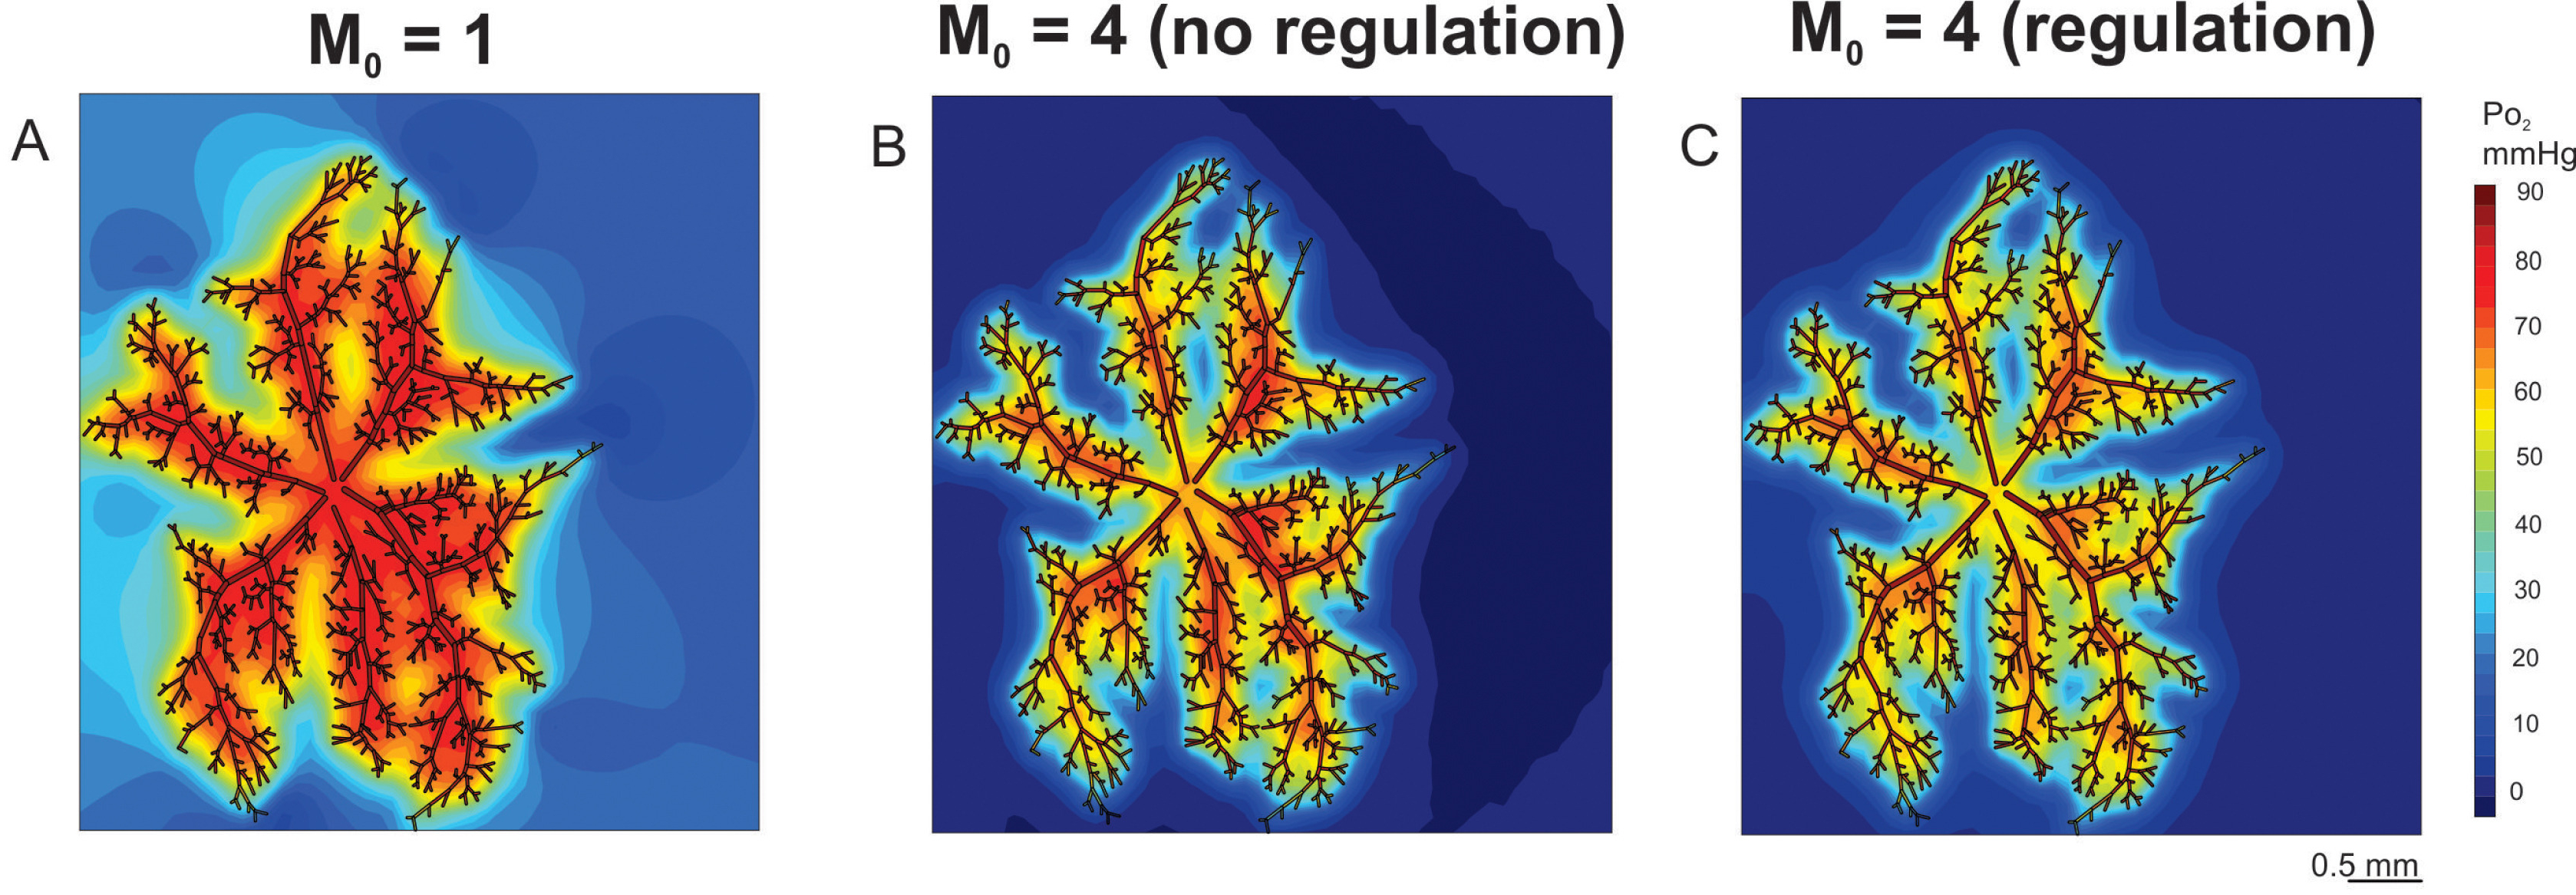
\includegraphics[scale=0.95]{Fry_et_al_2020_Fig_3_ABC}
\end{center}
\caption{Oxygen distribution (PO$_2$) within the arteriolar network and surrounding retinal tissue. Heatmaps are shown for low (A) and high (B and C) tissue oxygen consumption rates, $M_0$ (cm$^3$O$_2$/100cm$^3$/min), both with (C) and without (B) regulation (conducted metabolic response). Figure reproduced, with permission, from \citet{Fry_et_al_2020}.}
\label{Fig_Fry2020}
\end{figure}
%
%
\subsection{Retinitis pigmentosa}\label{Sec_RP}
%
Retinitis pigmentosa is a term used to denote a group of inherited retinal diseases that result in progressive vision loss~\cite{Hamel_2006,Hartong_et_al_2006}. RP typically presents as a rod-cone dystrophy, in which rod photoreceptors malfunction and die before cone photoreceptors, though the term is often used to encompass cone-rod dystrophies, in which cones are affected first, and rarer cases where both rods and cones are affected on a similar timescale~\cite{Hamel_2006,Hartong_et_al_2006}. In what follows, we shall focus largely on the rod-cone dystrophy form.

Rods degenerate because either they or the underlying RPE express a mutant gene; however, cones do not typically express a mutant RP gene, so the cause of cone death is unclear~\cite{Daiger_et_al_2007,Ferrari_et_al_2011,Hamel_2006,Hamel_2007,Hartong_et_al_2006,Roosing_et_al_2014}. Five complementary mechanisms have been proposed to explain secondary cones loss: 1.\ oxygen toxicity~\cite{Stone_et_al_1999,Travis_et_al_1991,Valter_et_al_1998}, 2.\ trophic factor depletion~\cite{Chalmel_et_al_2007,Leveillard_et_al_2004,Ait-Ali_et_al_2015}, 3.\ metabolic dysregulation~\cite{Punzo_et_al_2009,Punzo_et_al_2012}, 4.\ toxic substance release~\cite{Ripps_2002} and 5.\ microglia activation~\cite{Gupta_et_al_2003}. Thus far, mathematical models have been developed to explore the first four of these mechanisms. These studies demonstrate an important strength of mathematical modelling, namely its utility in isolating mechanisms in ways that would be difficult, if not impossible, experimentally.

Roberts et al. have developed reaction-diffusion PDE models for the oxygen toxicity (1D and 2D~\cite{Roberts_et_al_2017,Roberts_et_al_2018a}) and trophic factor (1D~\cite{Roberts_2022a,Roberts_2022b}) hypotheses.
These models were the first to formally address the long-unanswered question as to which spatio-temporal patterns of retinal degeneration (and hence visual field loss), characteristically observed in RP patients, these mechanisms are capable of generating.
It was found that oxygen toxicity may account for a subset of these patterns (see Figure~\ref{Fig_Roberts2018}~\cite{Roberts_et_al_2017,Roberts_et_al_2018a}), while, under the simplest of assumptions, the trophic factor mechanism was unable to account for any of them~\cite{Roberts_2022a}.
Relaxing some of these assumptions, in particular, allowing the mutation-induced rod degeneration rate and cone susceptibility to trophic factor depletion to vary spatially, an inverse problem was solved, identifying biologically realistic conditions under which trophic factor depletion could recapitulate known patterns of retinal degeneration~\cite{Roberts_2022b}.
These models were also used to determine the conditions under which patches of retinal degeneration will expand or remain stable, and to predict the effects of treatment with antioxidants and trophic factors~\cite{Roberts_2022a,Roberts_et_al_2017,Roberts_et_al_2018a}.
%
\begin{figure}
\begin{center}
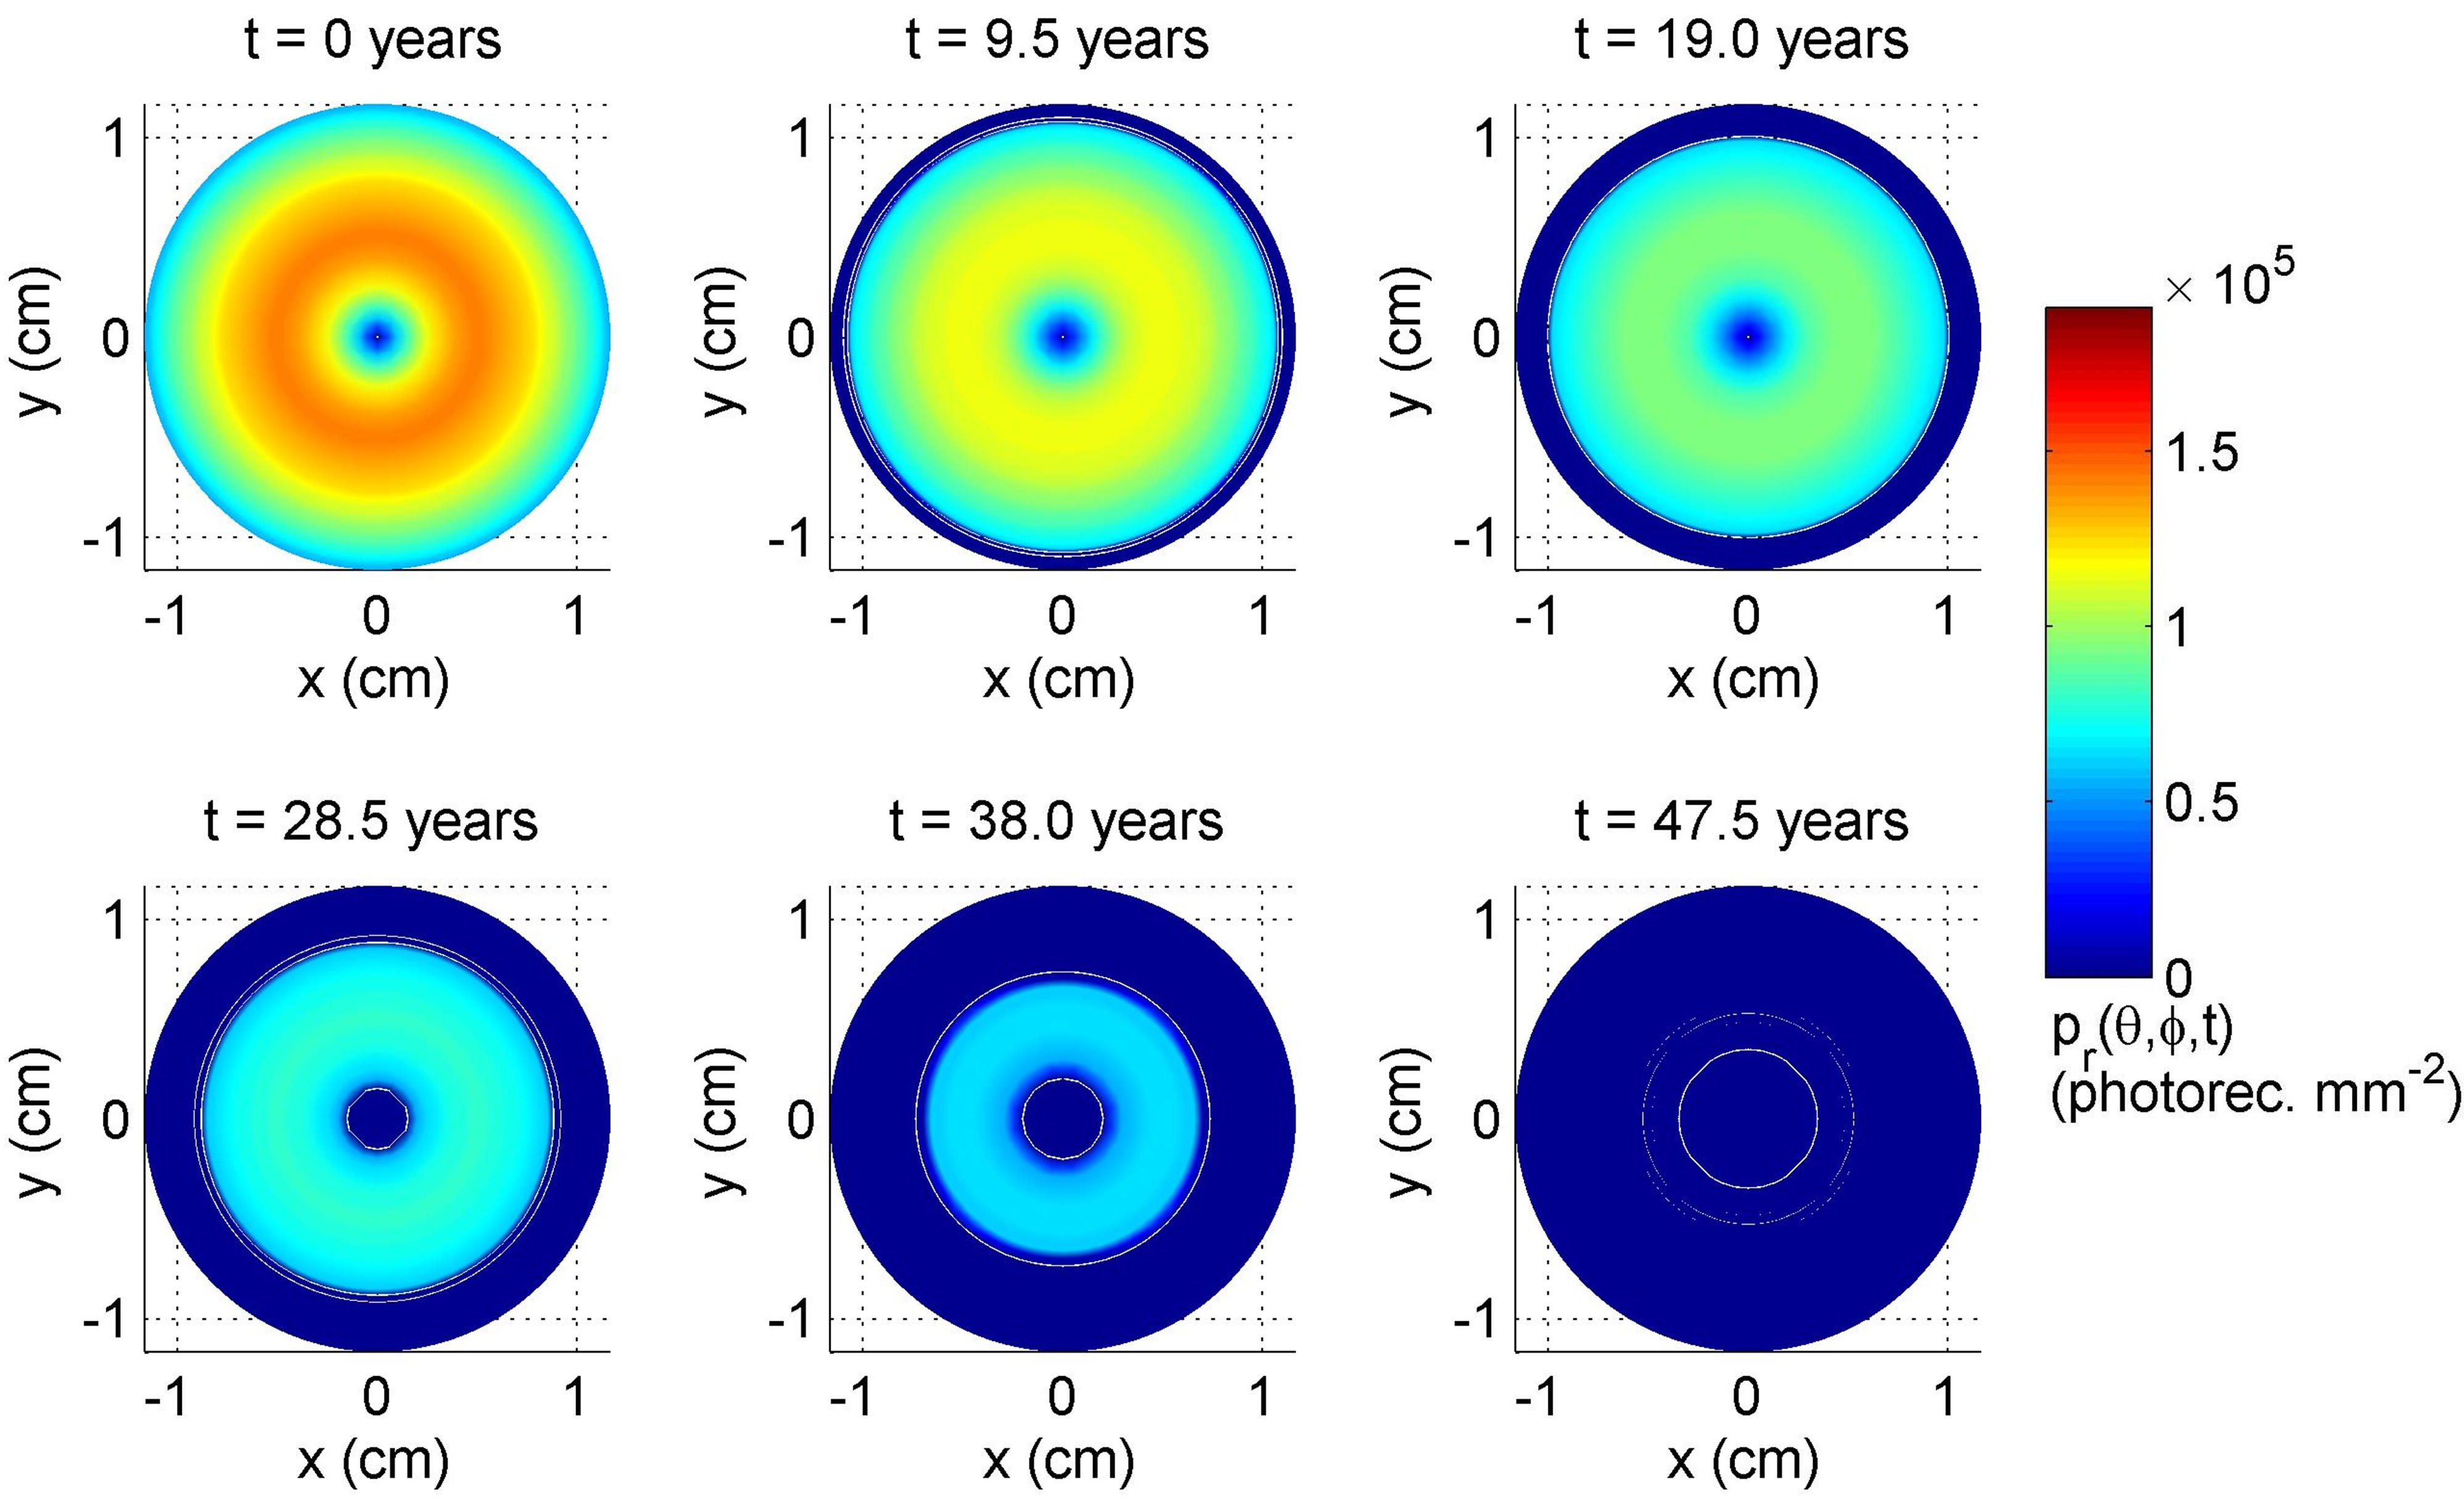
\includegraphics[scale=0.24]{Roberts_et_al_2018_Fig_5_a}
\end{center}
\caption{Exemplar spatio-temporal pattern of rod degeneration in RP, generated by the oxygen toxicity mechanism (the cone degeneration pattern is identical). The model replicates a classic pattern of retinal degeneration in RP, incorporating degeneration expanding inwards from the retinal periphery (ora serrata) and outwards from the parafoveal/perifoveal region. Figure reproduced, with permission, from \citet{Roberts_et_al_2018a}.}
\label{Fig_Roberts2018}
\end{figure}
%

Camacho et al. have constructed a range of well-mixed and compartmental ODE models, each exploring one or both of the trophic factor depletion and metabolic dysregulation hypothesis, under both healthy and RP conditions. Under healthy conditions, their models replicated the rhythmic variation in rod and cone outer segment length observed \emph{in vivo}~\cite{Camacho_et_al_2010,Camacho_et_al_2016b,Colon_Velez_et_al_2003, Wifvat_et_al_2021}. Further, these models predicted conditions under which rods and cones can stably coexist, revealing that the assistance provided to the cones by the rods via a trophic factor is crucial in this respect~\cite{Camacho_et_al_2010,Camacho_et_al_2016b,Colon_Velez_et_al_2003, Wifvat_et_al_2021}. This group’s retinal metabolic models are the most biochemically detailed to have been generated to date, using sensitivity and bifurcation analyses to determine which processes are most important in maintaining a healthy homeostasis~\cite{Aparicio_et_al_2022,Dobreva_et_al_2022,Camacho_et_al_2019,Camacho_et_al_2021a}. Under RP conditions, their models clarify and elucidate the stages of retinal degeneration that may be traced on the road to complete atrophy, highlighting which processes must change to allow progression to the next stage~\cite{Camacho_and_Wirkus_2013,Camacho_et_al_2016,Camacho_et_al_2016c}. Further, they apply optimal control theory to identify optimal treatment strategies under various constraints~\cite{Camacho_et_al_2014,Camacho_et_al_2020}.

Lastly, Burns et al. have formulated a 1D hybrid model for the toxic substance hypothesis, containing both continuous-deterministic and discrete-stochastic elements~\cite{Burns_et_al_2002}. This model is effective in capturing the initial patchy loss of photoreceptors observed in RP, and is also capable of replicating the exponential decline in photoreceptor numbers measured in RP mouse models~\cite{Clarke_et_al_2000}.
%
\subsection{Non-neovascular AMD}\label{Sec_non-nAMD}
%
The retinal disease AMD can be divided into three stages: early, intermediate and late~\cite{Ferris_et_al_2013}. The early and intermediate stages are distinguished by the development of pigmentary abnormalities and the size of cholesterol-rich deposits known as drusen (singular, druse) which form between the RPE and BrM (hard and soft drusen), and between the RPE and photoreceptors (reticular pseudodrusen/subretinal drusenoid deposits), while the late stage may be characterised as dry or wet~\cite{Coleman_et_al_2008,Ferris_et_al_2013,Jager_2008,Wu_et_al_2022}. Non-neovascular AMD (non-nAMD), considered in this section, consists of the early and intermediate stages, together with the dry form of the late stage (see Section~\ref{sec:RetinalHaemodynamicsNAMDDR} on nAMD)~\cite{Ferris_et_al_2013}. In the dry late stage, the central retina and choroid degenerate in a process known as geographic atrophy (GA)~\cite{Coleman_et_al_2008,Jager_2008,Ly_et_al_2016}.

A number of mechanisms have been suggested to drive non-nAMD including oxidative stress, drusen accumulation, cholesterol accumulation and lipofuscin accumulation~\cite{Ambati_and_Fowler_2012,Handa_et_al_2019}. Mathematical models have been developed to consider each of these mechanisms and this area has great potential for future modelling studies~\cite{Handa_et_al_2019,Luthert_et_al_2018}.

\citet{Mazzitello_et_al_2009} and \citet{Family_et_al_2010} constructed a simple stochastic model for the accumulation of lipofuscin, a chemical which builds up within RPE cells and may eventually prove toxic to them~\cite{Sparrow_and_Boulton_2005}. They capture the aggregation of  lipofuscin granules, though they do not link this to RPE cell death.

\citet{Zekavat_et_al_2017} and \citet{Scheepers_et_al_2020} have developed compartmental ODE models for drusen and cholesterol accumulation. The models capture features such as the build-up of drusen and their macrophage-mediated elimination, and determine regions of parameter space in which a healthy homeostasis may be maintained.

\citet{Linsenmeier_and_Zhang_2017} and \citet{McHugh_et_al_2019} have developed 2D and 3D PDE models (respectively) to predict the effects of soft and hard drusen upon retinal oxygen distribution (see Figure \ref{Fig_LinZhang2017}). It was found that it is the size of a druse, rather than the diffusivity of oxygen within a druse, which has the greatest effect on photoreceptor oxygenation, and that wide (soft) druse are more likely to cause photoreceptor hypoxia (oxygen starvation) than tall (hard) druse. Further, \citet{Vercellin_et_al_2021} have constructed a 2D PDE model predicting the effects of reduced blood flow on central retinal oxygenation, identifying the most vulnerable regions.
%
\begin{figure}
\begin{center}
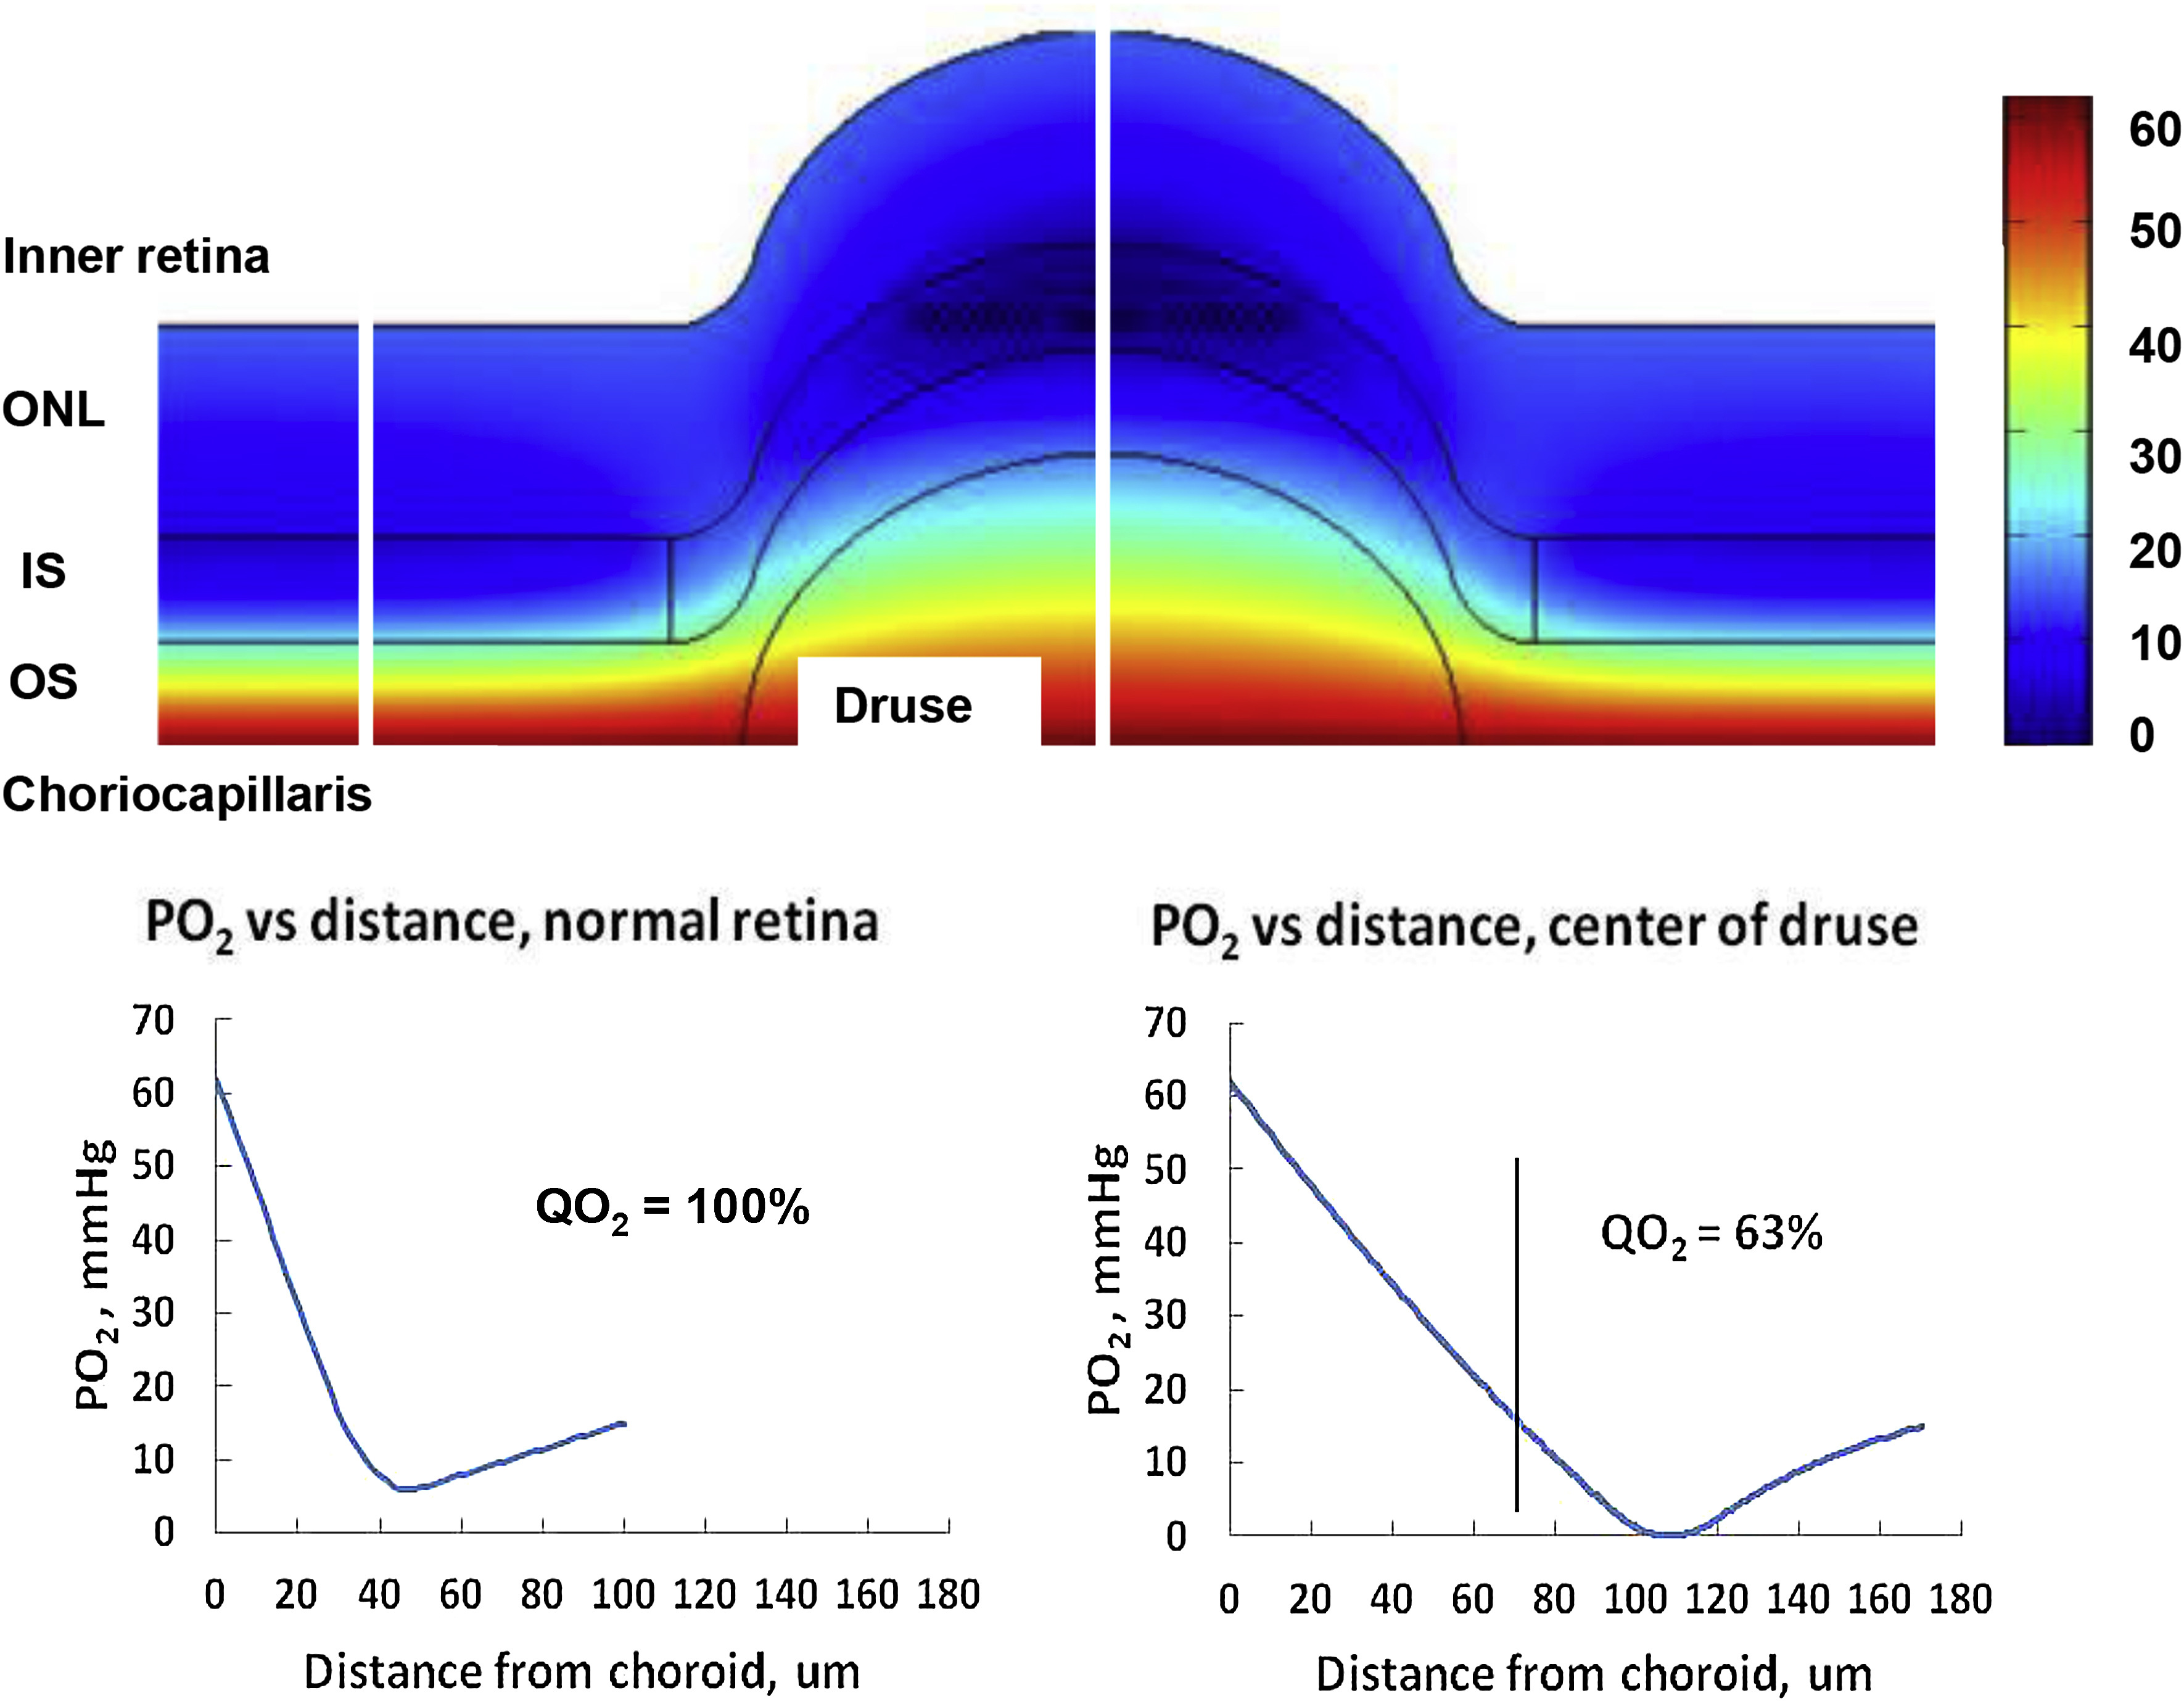
\includegraphics[scale=0.9]{Linsenmeier__and_Zhang_2017_Fig_21}
\end{center}
\caption{Oxygen profile (PO$_2$) through the outer retina in the presence of a large druse. Top panel: 2D heatmap showing the oxygen profile across normal and druse-containing retinal regions. Bottom panels: 1D profile through the normal (left) and druse-containing retinal regions (right). Figure reproduced, with permission, from \citet{Linsenmeier_and_Zhang_2017}. Abbreviations --- OS: outer segment, IS: inner segment, ONL: outer nuclear layer.}
\label{Fig_LinZhang2017}
\end{figure}
%

Lastly, \citet{Shen_et_al_2020} formulated a simple phenomenological model to predict GA progression based upon measurements of GA propagation rates within the literature. The model is successful in replicating some of the patterns seen \emph{in vivo}, though it is not capable of explaining the mechanisms behind these patterns.
%
%




\section{Drug delivery to the retina}\label{sec:DrugDelivery}

In this section we review models aimed at optimising or developing drug delivery techniques for the treatment of retinal diseases.
Ocular drug delivery, including delivery to the retina, has recently been reviewed elsewhere from a computational fluid dynamics point of view~\cite{Bhandari_2021}.
Thus, this section will focus on models that were not covered in said review.

\subsection{Intravitreal injections}

\textit{In silico} models of the PK and PD of anti-VEGF molecules, mainly administered inside the vitreous, have been discussed in Section~\ref{sec:Anti-VEGF}.
Here, we focus more specifically on models aimed at understanding and optimising the surgical procedure of injecting drugs in the vitreous humour and how the outcome may be affected by the eye's characteristics.

The effects of injection parameters such as needle shape, angle of insertion and speed of injection may affect the delivery of drug to the retina and are hard to assess \textit{in vivo}.
Several models have been developed to identify those effects using finite element meshes which realistically capture the geometry of the eye.
Some studies assume the initial dose to be spherical with drug concentration equal to the dose~\cite{Friedrich_1997,Friedrich_1997a}.
In these studies, the initial location of the dose was demonstrated to affect the the time taken to clear the drug from the vitreous by almost four-fold for the configurations tested~\cite{Friedrich_1997}.
However, flow in the vitreous was neglected.
Therefore, drug transport was solely due to diffusion and thus strongly dependent on the dose~\cite{Friedrich_1997}.

Needle type, injection speed and needle penetration angle were accounted for to describe the initial concentration profile in another finite element model of the human eye~\cite{Jooybar_2014}.
In this model, the drug was transported by flows in the vitreous as well as by diffusion.
Furthermore, injection parameters affected the shape of the initial drug distribution, although the needle was not modelled explicitly.
The model showed significant sensitivity to the injection parameters on the exposure of the macula to the drug.
Slower injections and larger needle gauge were shown to increase the concentration peak at the macula by an order of magnitude compared to a model assuming a spherical initial distribution of the dose.
Unsurprisingly, penetration angle strongly affects the concentration peak --- by up to \SI{80}{\percent} at the macula~\cite{Jooybar_2014}.
This model showed the importance of considering advective transport of intravitreally injected drugs. 

Injection parameters may also influence the risks of complications due to the procedure.
By modelling the eye, the needle and their mechanical interactions, including deformation of the cornea, it was found that an angle of \SI{45}{\degree} between the needle and the optical axis was ideal to minimize complications~\cite{Karimi_2018}.
To draw this conclusion, the authors assumed that post injection complications were correlated with the maximal principal stress, namely the normal stress on a plane subject to no shear stress.  
The increased stress caused by insertion angles closer to the vertical or horizontal axis seem to correlate with experiments which reported more injuries at those angles~\cite{Karimi_2018}.

The aging vitreous humour undergoes changes causing its liquefaction~\cite{Los_2003}.
Furthermore, in disease, vitrectomy may be performed to replace the vitreous humour by a substitute gel or oil in order to lower pathological traction at the interface with the retina~\cite{Dervenis_2022}.
Alterations in the properties of the vitreous humour, or its substitutes, has been investigated computationally with finite element models, where drug transport is modelled by advection-diffusion equations~\cite{Kathawate_2008,Modareszadeh_2012}.
Point sources for the injection of the dose are used in these studies.
The earliest model investigated the possibility of toxic levels of drugs in the retina~\cite{Kathawate_2008}.
The model showed that the exposure of the retina increases strongly in configurations with low diffusivity of the drug and low viscosity of the vitreous substitute, due to convection overtaking diffusion~\cite{Kathawate_2008}.
Shifts to predominantly convective transport of drug have been showed to occur due to saccadic movements typical of vitrectomised eyes~\cite{Modareszadeh_2012}.
The finite element model showed that higher movement amplitude hastens the spread of the drug within vitreous humour substitutes.
While homogenisation of drug concentration was reported to happen on a time scale of days, this may reduce to the order of minutes in vitrectomised eyes~\cite{Modareszadeh_2012}.
Furthermore, it was shown that the diffusion coefficient of the drug had limited impact on its spread in the vitreous after the first few minutes~\cite{Modareszadeh_2012}.

More recently, saccadic movement effects on intravitreally injected drugs have been simulated in a vitreous liquefied with age~\cite{Ferroni_2020}.
This model predicted that, in the presence of saccades, the drug concentration homogenised throughout the vitreous in less than a minute, where it would take about a day in the absence of saccades.
Interestingly, it has been shown computationally that in locally liquefied vitreous (e.g., a substitute for the vitreous inserted surgically), fluid flow converges towards the liquefied region as it offers less resistance~\cite{Khoobyar_2022}.
This result is of interest in understanding the kinetics of intravitreally injected drugs, especially larger ones such as anti-VEGF which are more subject to convection.

\subsection{Implants/port-delivery}

A number of models, including those discussed above, have been used to compare the efficacy of drug delivery to the vitreous by an injection or by a controlled release from a system implanted in the eye, typically in the vitreous or on the outer surface of the sclera~\cite{Jooybar_2014,Kathawate_2008,Kavousanakis_2014,Park_2005}.
Overall, these comparisons highlight the capacity of controlled release systems to prolong the drug availability in ocular tissue.
However, those models were not concerned with the mechanisms of drug delivery from those implants but rather assumed empirical release rates.

Understanding of the degradation process of vitreal implants is essential to control drug release.
The effects of altered vitreous on this process have been modelled, coupling the degradation process of the implant to drug transport in the vitreous and retina~\cite{Ferreira_2020}.
Drug distribution profiles were simulated for two different vitreous humour substitutes, namely a silicone oil and a saline solution.
The authors concluded that silicone oil substitutes could delay the degradation of the implant and provide higher mean concentration in the retina.
By comparison, the saline solution substitute showed similar or lower concentrations compared to non-vitrectomised eyes~\cite{Ferreira_2020}.

In the model by Li et al., the drug molecules are trapped within the mesh structure of a hydrogel, represented as a sphere~\cite{Li_2022a}.
Unlike the previous chemical degradation of the implant, degeneration of the hydrogel corresponds to loosening of the mesh over time, described as an empirical exponential law.
Both the initial location and properties of the hydrogel were varied.
Perhaps unsurprisingly, while the location did not affect the depletion of drugs within the hydrogel, positioning the hydrogel closer to the target site, e.g., the macula, caused higher and earlier peaks in concentration.
However, higher peaks implied quicker clearance from the macula and therefore concentrations reach similar levels to other implantation sites within two weeks~\cite{Li_2022a}.
Hence, the location of the hydrogel has to be chosen wisely as to not induce toxicity while maintaining therapeutic levels of drug within the retina.
In contrast, the hydrogel properties tested did not show a significant effect on macular concentrations, though tighter meshes cause a delay in the release of the drug.

Recently, a PK model specific to anti-VEGF molecules in the vitreous and aqueous humour, released from degrading spheres, has been simulated and validated against experimental data~\cite{Heljak_2022}.
Note that, unlike some of the PK models of anti-VEGF described in the previous section, these models did not ignore convective transport in the vitreous or the other ocular tissues.
Rather, these tissues are considered as porous mediums through which transport is driven by diffusion and a pressure gradient between the IOP in the anterior part of the eye and the lower pressure at the sclera~\cite{Ferreira_2020,Ferreira_2018,Heljak_2022,Khoobyar_2021,Li_2022a}.
In their noteworthy study, Khoobyar et al. determine the depletion of drug from an implant~\cite{Khoobyar_2022}.
Through rigorous mathematical analysis of a simplified drug transport model, they derived an analytical formulation for the estimated half-life of an implant in the vitreous which depends on the ratio of convective mass transfer to diffusivity.
However, this estimate is valid only when diffusive transport dominates over convective transport.



The same equations can be used to describe the transport of molecules from the sclera to the vitreous, a scenario corresponding to implants inserted on the outer surface of the sclera.
The case of a drug diffusing through such an implant to enter the sclera, later reaching the choroid and retina, was modelled \textit{in silico} recently~\cite{Abootorabi_2021}.
The clearance through choroidal and retinal circulation was accounted for and simulations showed very good agreement with data.
The model revealed the influence of the implants porosity on the controlled release of drugs and suggested parameters that could be tailored to individual needs~\cite{Abootorabi_2021}.
Kotha and Murtom\"aki also modelled drug release from a scleral implant, with the difference that choroidal blood flow was modelled explicitly~\cite{Kotha_2014}.
The influence of diffusion coefficients in the sclera as well as the permeation coefficients regulating exchanges between each layer of tissue were quantified and demonstrated complex relationships between the parameters and the efficacy of the implant.

Of particular relevance to scleral implants are the retinal barriers to drug.
The role of these barriers, namely the RPE-BrM complex, choroidal and retinal circulation, and the ILM, has been investigated \textit{in silico}.
Active transport by the RPE, along with clearance from the inner retinal blood vessels, were included in a model by Causin et al~\cite{Causin_2016}.
The permeability of the blood vessels walls was shown to have little influence on clearance, though it is suggested by the authors that this could be a consequence of the simplifying assumptions made concerning mass transport between the retina and its vasculature.
In contrast, active transport by the RPE was found to have a significant impact on drug concentration in the retina and vitreous.
Other models came to the same conclusion, despite this specific transport mechanism being modelled differently~\cite{Balachandran_2008,Kotha_2014}.
Despite this evidence, active transport across the RPE has generally been neglected in PK models of IVI and controlled-release devices.


\subsection{Subretinal, periocular and systemic administration}

While accumulating evidence suggests otherwise, the retina and the eye in general are thought to be isolated from systemically injected drugs, on account of the numerous biological barriers separating the eye and retina from the rest of the body.
Therefore, systemic, or intravenous, administration of drugs for treatment of retinal pathologies remain uncommon.
Accordingly, few modelling works have been published on the matter.
However, understanding of the PK of intravenously injected drugs remains of interest since harmful effects on the retina have been reported~\cite{Fu_2017}.

In fact, significant ocular exposure, determined by a non-compartmental model (a type of model where the whole body is considered as a single homogeneous compartment), to intravenously injected antibodies has been reported~\cite{Shivva_2021}.
The possibility of deducing vitreous concentrations after intravenous injection has been demonstrated by a compartmental model~\cite{Vellonen_2015}.
However, the transfer rate from systemic circulation to the eye compartment was taken from a previous model describing the rate of clearance from the eye compartment into the systemic circulation, which may differ from the clearance rate in the opposite direction.
The same model applied to the analysis of experimental data on the permeability of the outer blood-retinal barrier found asymmetric exchange rates between the choroid and the vitreous~\cite{Ramsay_2019}.
Additionally, the analysis suggests that the RPE may not be the main route of clearance from the vitreous for drugs entering the retina via the systemic circulation~\cite{Ramsay_2019}.

In contrast, injections into the subretinal space have gained traction, especially for the delivery of cell or gene therapies.
Subretinal injections provide direct access to the targeted cells, namely the photoreceptor and RPE cells.
In both cases, the blood-retinal barrier plays an important role in the total exposure of the tissue to the therapeutics.
Yet, the mechanisms of exchange between systemic circulation and the retina remain elusive and few \textit{in silico} models of subretinal or systemic administration of ocular drugs have been developed.
A computational fluid dynamics model for the transport of molecules across the RPE was developed and calibrated with an \textit{in vitro} experimental setup~\cite{Davies_2020}.
Despite active transport not being considered in the model, this work provides a validated framework which can be built upon to incorporate such dynamics and to determine key RPE parameters.

Injection of anti-VEGF under the sclera (periocular), as a safer and less invasive alternative to the intravitreal route, is another promising technique.
This method would also benefit from understanding of the ocular barriers.
A one-dimensional, time-dependent, diffusion model was developed to simulate the transport of a protein across those layers in the mouse eye after periocular injection~\cite{Gabhann_2007}.
The diffusivity of each layer was estimated based on the fraction of extracellular space, while permeability of the barriers and clearance rates were fitted to experimental data.
The model demonstrated it takes only 75 minutes for most of the injected dose to enter the eye and 95 minutes for it to be cleared, with over \SI{99}{\percent} of the clearance happening through the choroidal and episcleral circulations.
Compared to simulated IVI, periocular injections showed a two-fold higher peak concentration in the retina.
However, the peak persists longer with IVI.
Similar work modelling injections of anti-VEGF molecules into the space between the choroid and the sclera showed that the clearance rate from the episclera was negligible for large molecules~\cite{Zhang_2018}.
However, it may still play a role for smaller molecules such as the fluorescent protein simulated in the previous model~\cite{Gabhann_2007}.

Of potential interest to the reader are two models of topical delivery and spray systems~\cite{Mori_2017,Nweze_2020}.
Modelling work of these techniques remains scarce but the growing interest for, e.g., cell and gene therapy may motivate modellers in the coming years.



\section{\textit{In silico} clinical trials in the retina}\label{sec:InSilicoTrials}

The previous sections have detailed the vast literature that deals with modelling retinal haemodynamics, oxygenation, disease and the impact of drugs in both healthy and diseased retinas. 
However, there is currently very little research on formalising these models within the framework of \textit{in silico} clinical trials (ISCTs). 
ISCTs are simulations of clinical trials to test medical devices or drugs with the aim of eventually being used as digital evidence to reduce, refine and replace animal and human participants in preclinical and clinical experiments~\cite{Viceconti2021a}. 
At each stage of clinical trials (preclinical, Phase I, II, III), ISCTs can be used: for early proofs-of-concept in the drug development phase; to simulate greater numbers of patients in each phase, hence representing greater biological variability in the trial; to augment trials such that fewer real-world patients are required; to run numerous trials that can optimise an intervention that would not be possible in reality; as well as to investigate rare events that might not occur in a real-world trial~\cite{Pappalardo2019, Viceconti_2016, Viceconti2017}. 
Another crucial aspect of an ISCT is the ability for a patient to act as their own control simulation-wise, introducing a new potentially more impactful/patient-specific way of running clinical trials.

The paradigm of an ISCT is very similar to that of a real-world clinical trial except the disease, intervention and trial setup are simulated. 
ISCTs require virtual populations of the disease of interest, a mechanistic model of the disease and treatment using the proposed intervention, and a statistical analysis plan that will analyse the output of the trial~\cite{Alfonso2020}. 
Figure~\ref{fig:ISCT} depicts a general schematic of how an ISCT might run for nAMD drug testing.

\begin{figure}[t!]
  \centering
  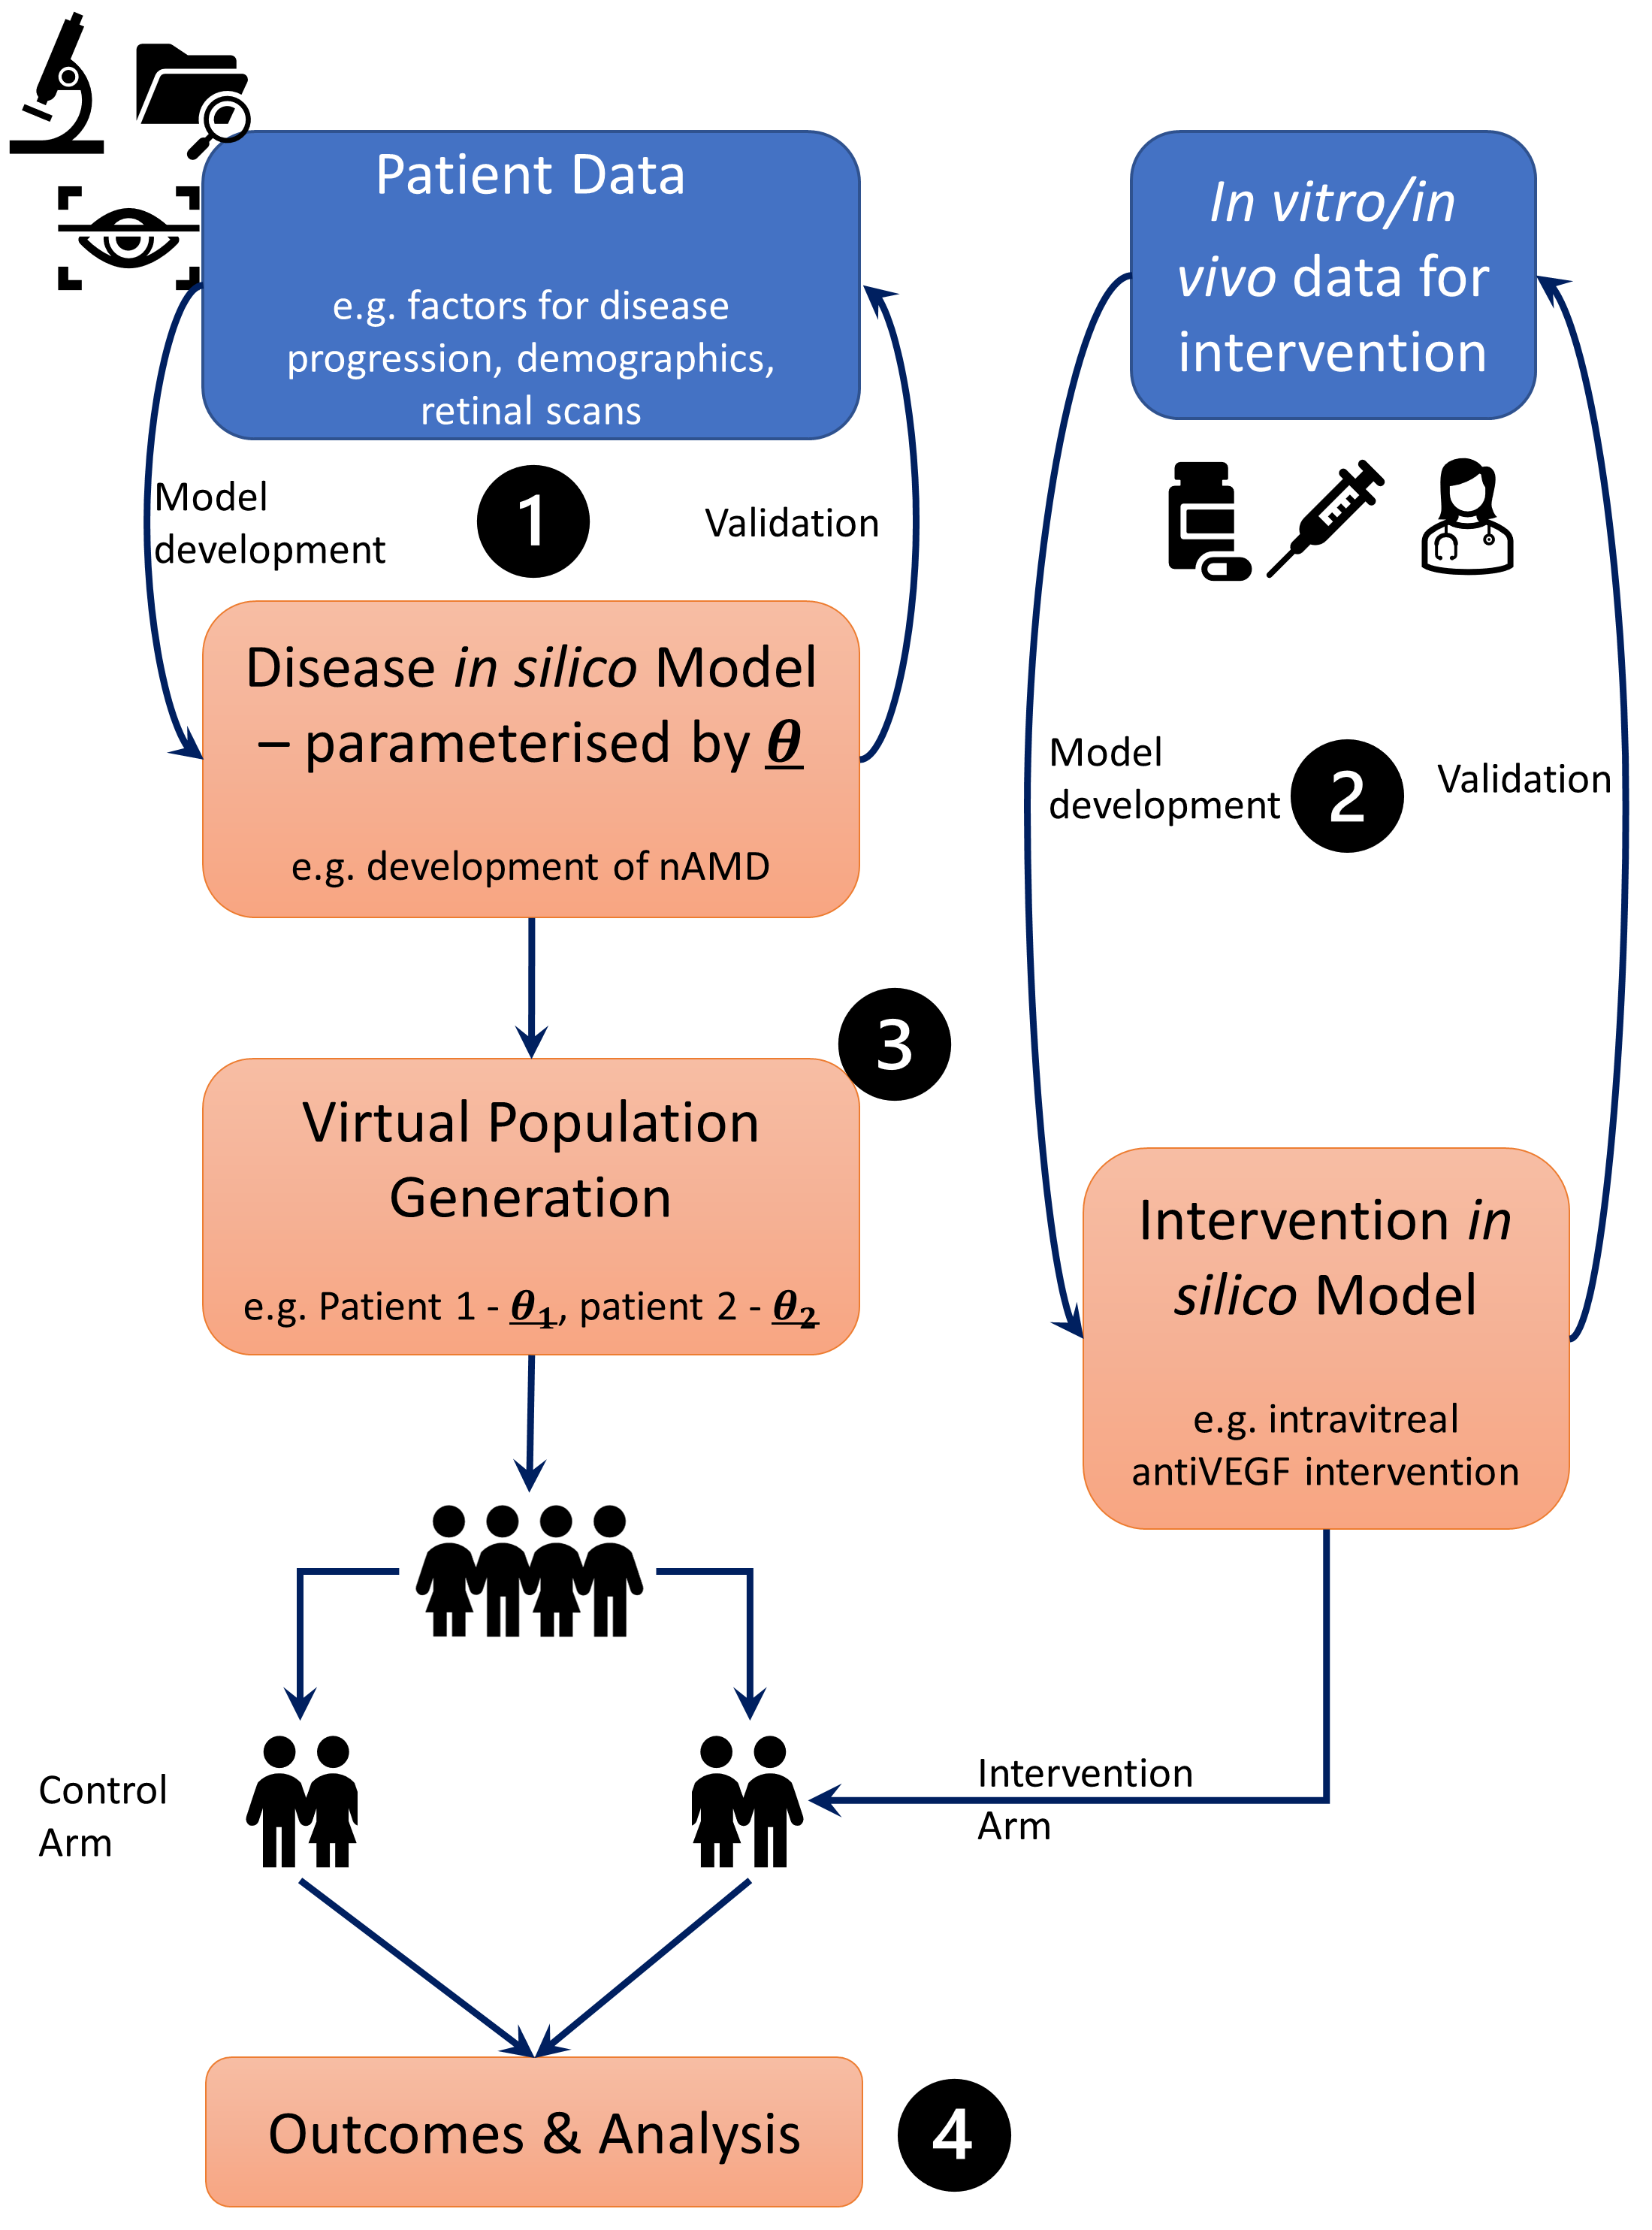
\includegraphics[width=1\textwidth, height=9.3cm]{Fig_sec_8.png}
  \hfill
  \caption{Schematic of a generic ISCT with an example of nAMD drug testing. 1) \textit{In silico} model development of disease with validation loop linked to patient data. 2) \textit{In silico} model development of intervention with validation loop linked to \textit{in vitro} and \textit{in vivo} data. 3) Virtual population generation using the disease model parameters. 4) ISCT run on intervention and control arms with appropriate outcomes and analysis.}
  \label{fig:ISCT}
\end{figure}

\subsection{Mechanistic models of disease and intervention}

The central aspect of any ISCT is the mechanistic model that predicts the outcome of an intervention (or lack thereof). 
This is equivalent to the administration of the intervention in a real-world clinical trial. 
The mechanistic model is one that is based on the underlying physics and chemistry of the system being investigated. 
This model will usually simulate a disease, for example nAMD~\cite{Hoyle_2017}. 
The intervention is then also simulated, in this case anti-VEGF therapies. 
Both the disease model and intervention model must be validated against \textit{in vitro} or \textit{in vivo} data in order to be used in an ISCT (Figure~\ref{fig:ISCT}).

Examples of disease/intervention models that have been developed include coronary stent models for occlusive heart diseases~\cite{Antonini2021, Berti2021}, insulin control algorithms in Type 1 diabetes~\cite{Kovatchev2009}, non-pharmaceutical interventions on respiratory tract interventions~\cite{Arsene2022}, bone morphogenetic treatment in paediatric orphan bone disease~\cite{Carlier2018}, anaemia treatment in haemodialysis patients~\cite{Fuertinger2018}, warfarin in atrial fibrillation patients~\cite{Ravvaz2017}, cancer vaccines on lymph node cancers~\cite{Gaffney2022}, targeted delivery of drugs in patients with covid-induced pneumonia~\cite{Wang2022}, mematine treatment of Alzheimer’s disease~\cite{Swietlik2022}, flow diverters in intracranial aneurysms~\cite{SarramiForoushani2021}, predicting pro-arrhythmic cardiotoxicity in cardiomyocytes~\cite{Passini2017}, and thrombectomy/thrombolysis for acute ischaemic stroke~\cite{Konduri2020}, amongst many more.

Within this review, we have also demonstrated the vast literature on \textit{in silico} models of retinal disease, ranging from non-nAMD and RP (Section~\ref{Sec_Ox_RP_non-nAMD}), to nAMD and DR (Section~\ref{sec:RetinalHaemodynamicsNAMDDR}), as well as models of intervention through intravitreal injections, implants, and sub-retinal injections (Section~\ref{sec:DrugDelivery}).
This has laid the groundwork, furnishing models which can be adapted into the ISCT paradigm. Despite the rapidly growing literature on ISCTs in various disease conditions, little or no papers have been published on applying this paradigm to diseases of the retina.

Once a mechanistic model of disease and intervention has been established and extensively validated, the next step is to generate virtual populations with this disease that can be used in the ISCT.

\subsection{Virtual Populations}

To run clinical trials, sub-populations of the target population are required. A crucial first step is therefore to generate virtual populations (VPs) of the disease of interest that will eventually be used in the \textit{in silico} clinical trials. For example, if an intervention for nAMD patients is to be tested \textit{in silico}, a population of nAMD patients is required.

Virtual population generation is a nascent and rapidly developing field. In essence, a virtual patient is one with a specific set of parameters for a given disease model. Virtual populations are therefore sets of patients with parameters that reproduce the statistics of interest of the clinical population of interest~\cite{Allen2016}.

One simple method of generating VPs is to assume a Gaussian distribution for each model parameter that will be patient specific. 
For each patient, a parameter value will be drawn from these Gaussian distributions to represent that patient~\cite{Gaffney2022, Jenner2021}. 
The mean and standard deviation of the parameters can be adjusted to match empirically observed data either manually or through optimization~\cite{Alfonso2020}. Often, these patient parameters are not independent of each other – for example, sex and height are correlated. Therefore, more complex sampling strategies that maintains the relationships between patient parameters have been developed.

Bayesian statistics have been used extensively to generate patient parameter populations for the purpose of ISCTs. Haddad et al. generated VPs using a Bayesian framework for augmenting clinical trials, demonstrating decreased sample size and trial length would be required for the real-world trial when using these VPs~\cite{Haddad2017a}. For warfarin patients, a Bayesian model was used to generate VPs from a pre-defined dataset~\cite{Fusaro2013}. Other methods that have been used to generate VPs include vine copulas to generate virtual stroke populations~\cite{Miller2021}. Pezoulas et al. also used tree-based methods (supervised and unsupervised) to generate VPs for cardiomyopathy drug development~\cite{Pezoulas2020} but found that Gaussian Mixture Models with Variational Bayesian Inference outperformed supervised tree ensembles when comparing the VPs to the data~\cite{Pezoulas2021}.

As a virtual patient is effectively a set of parameters for the mechanistic model that represent a given individual, this can also be extended to 3-dimensional models of arteries or other physiological organs – where now the parameters might represent curvature of vessels, degree of stenosis or material properties of the artery. 
This introduces an added difficulty of modifying the computational mesh for each virtual patient.
Because of this, most ISCTs involving patient meshes generate the mesh from patient-specific image data and simulate variability through variation in, for example, orthopaedic implant positioning~\cite{AlDirini2019}, plaque growth over time on the arteries~\cite{Pleouras2021}, and blood pressure and thrombus formation parameters applied on the mesh~\cite{SarramiForoushani2021}. 
However, statistical shape modelling is increasingly being used to generate VPs of the meshes themselves~\cite{Rodero_2021}

VPs of retinal disease have yet to be extensively used in the literature. With appropriate data, however, VPs can be generated using the techniques documented.

\subsection{Running the ISCT}

Once the mechanistic model and VPs have been developed, the ISCT protocol should be pre-defined – with a statistical plan, pre-defined primary and secondary outcomes, and trial inclusion and exclusion criteria. Current medical studies publish their protocols, with randomised clinical trials following the CONSORT guidelines~\cite{Schulz2010}. Once the study protocol is in place, the ISCT can be run and analysed with the pre-defined methodology.

Unlike real-world trials, the benefit of running an ISCT is the ability to run any permutation of trial you like, without consideration for cost or ethics. This allows for deeper investigation of the intervention in various sub-populations, helping to optimise the application of the intervention.

The validity of the mechanistic model and ISCT is an important factor in translating this paradigm to bedside use. Guidelines have been published by the American Society of Mechanical Engineers, `Verification \& Validation 40 Assessing Credibility of Computational Modeling through Verification and Validation: Application to Medical Devices'. These guidelines use a risk-informed credibility assessment, where the risk of the model defines how close the validation needs to be to real-world observations~\cite{ASME2018}.

Validation, verification, and uncertainty quantification (VVUQ) are necessary to give confidence in the models and ISCTs. Validation of the model depends on the context-of-use of the model and what risk is involved with its use, with higher risk models requiring higher validity~\cite{Pappalardo2019}. Validity of the VPs should also be considered (external validity) – the VPs should be representative of the wider population of interest for that disease i.e. not constrained by overly stringent exclusion criteria. Similarly, the ISCT should have ecological validity, where the results translate to real-life settings in which the trial results will be applied. 
Recent research has looked at simulating hospital environments stochastically to determine ecological validity of the ISCT~\cite{Fuertinger2018}.

Verification of a model verifies that the numerical implementation is correct and sufficiently accurate for the intended use.
This is often done by using the code to solve a problem where the solution is known i.e. an analytical solution exists.
Verification methods are usually well established for given models and their numerical implementation~\cite{Curreli2021, Pappalardo2019}. 
Uncertainty quantification is also an essential step. 
This includes both aleatoric uncertainty (uncertainty in the data used to inform a model) and epistemic uncertainty (uncertainty in the knowledge of the physiological system used to build the model), as well as numerical uncertainty when solving approximated mathematical equations computationally. 
All of these uncertainties must be quantified to ensure that a good comparison with real-world data can be made.


\section{Discussion}\label{sec:Conclusion}

% \subsection{Gaps in ISCTs for the retina}
Throughout this paper, we have reviewed the state-of-the-art models of the retina in both healthy and diseased conditions.
\textit{In silico} models have shed light on the interplay between biological mechanisms, such as autoregulation, necessary to maintain a healthy retina.
In addition, they have provided us with quantitative understanding of the range of insults that the retina can withstand.

Further, models have brought insights on the underlying mechanics of common retinal diseases, some of which may have been overlooked by traditional \textit{in vivo} and \textit{in vitro} investigation because of the difficulty of direct measurements.

Additionally, we have introduced the concept of \textit{in silico} clinical trials and the main components they require. 
Most of the building blocks for running an ISCT in the retina are already in place. When it comes to nAMD, there are already mechanistic models in place for the disease and intervention~\cite{Hoyle_2017, Vega2021}. However, two main gaps still exist that are required to run successful ISCTs in retinal disease: 

\begin{enumerate}
\item{Patient data linkage for comprehensive VP generation. For representative and valid VPs, imaging data needs to be linked to primary and secondary health records to give a comprehensive disease populations~\cite{ElBouri2021}.}

\item{Most clinical trials for retinal disease use visual acuity as a primary outcome, yet there is no \textit{in silico} model that reliably links visual acuity to the disease. This is the main stumbling block that needs to be addressed if ISCTs are going to be used extensively in retinal disease.}
\end{enumerate}

Whilst the future is incredibly promising for ISCTs, it is unlikely they will ever replace clinical trials. However, they can help refine and accelerate trials by eliminating pre-clinical testing, targeting an intervention to specific sub-populations or improving an intervention through repeated \textit{in silico} trial testing.


\bibliography{bibliography}{}

\end{document}